\documentclass[a4paper]{article}

% CUSTOM maketitle
\makeatletter
 \def\@maketitle{%
  \newpage
  \null
  \vskip 1.em
  \begin{center}%
  \let \footnote \thanks
    {\LARGE \bfseries\@title \par}%
    \vskip 1.em%
    {\large \langCourse \par}%
     {\large \langInstitute \par}%
    \vskip 1.em%
    {\large
      \lineskip .5em%
      \begin{tabular}[t]{c}%
        \@author { --- } \@istid \\
        {\href{mailto:\@email}{\tt\@email}}
      \end{tabular}\par}%
          \vskip 1.em%
    \ifx\@coadvisor\undefined      
        {\large \langAdvisor: \@advisor \par}%
    \else
        {\large \langAdvisor: \@advisor \par}%
        {\large \langCoadvisor: \@coadvisor \par}%
    \fi
    
  \end{center}%
  \par
  \vskip 1em}
\makeatother


% Commands to allow defining title, name, etc.
\makeatletter
\newcommand{\@StoreIn}[2]{ \gdef#1{#2} }
\newcommand*{\email}[1]{\@StoreIn{\@email}{#1}}
\newcommand*{\istid}[1]{\@StoreIn{\@istid}{#1\thanks{\langThanks}}}
\newcommand*{\advisor}[1]{\@StoreIn{\@advisor}{#1}}
\newcommand*{\coadvisor}[1]{\@StoreIn{\@coadvisor}{#1}}
\makeatother

% The 'utf8' package contains support for using UTF-8 as input encoding. 
\usepackage[utf8]{inputenc}
% The 'babel' package may correct some hyphenation issues of LaTeX. 
% Select your MAIN LANGUAGE for the Thesis with the 'main=' option.
\usepackage[english]{babel}
\usepackage{iflang}

% Solves some font enconding issues related to the output
\usepackage[T1]{fontenc}

% These packages are typically required. 
% Among many other things they add the possibility to put symbols in bold
% by using \boldsymbol (not \mathbf); defines additional fonts and symbols;
% adds the \eqref command for citing equations.
\usepackage{mathtools, amsmath, amsthm, amssymb, amsfonts}
\usepackage{nicefrac}
%

% Tikz  for creating graphics programmatically.
\usepackage{tikz}
\usetikzlibrary{shapes.geometric, arrows, positioning}

% These packages are most usefull for advanced tables. 
% 'multirow' allows to join rows throuhg the command \multirow which works
% similarly with the command \multicolumn.
% The 'colortbl' package allows to color the table (foreground and background)
% The package 'booktabs' provide some additional commands to enhance
% the quality of tables
% The 'longtable' package is only required when tables extend beyond the length
% of one page, which typically does not happen and should be avoided
\usepackage{array}
\usepackage{booktabs}
\usepackage{multirow}
\usepackage{colortbl}
\usepackage{spreadtab}
\usepackage{longtable}
\usepackage{pdflscape}
\usepackage{float}

% Set links for references and citations in document
\usepackage{hyperref}
\hypersetup{ colorlinks=true,
             citecolor=cyan,
             linkcolor=darkgray,
             urlcolor=teal,
             breaklinks=true,
             bookmarksnumbered=true,
             bookmarksopen=true,
}

% Provides better support for handling and breaking URLs.
\usepackage{url} 

% The package 'graphicx' supports formats PNG and JPG.
% Package 'subfigure' allows to place figures within figures with own caption. 
% For each of the subfigures use the command \subfigure.
\usepackage{graphicx}
\usepackage[hang,small,bf,tight]{subfigure}

\usepackage[format=hang,labelfont=bf,font=small]{caption} 
% the following customization adds vertical space between caption and the table
%\captionsetup[table]{skip=10pt}

% These packages are required for list code snippets.
\usepackage{xcolor}
\usepackage{color}
% The following special color definitions are used in the IST Thesis
\definecolor{forestgreen}{RGB}{34,139,34}
\definecolor{orangered}{RGB}{239,134,64}
\definecolor{lightred}{rgb}{1,0.4,0.5}
\definecolor{orange}{rgb}{1,0.45,0.13}	
\definecolor{darkblue}{rgb}{0.0,0.0,0.6}
\definecolor{lightblue}{rgb}{0.1,0.57,0.7}
\definecolor{gray}{rgb}{0.4,0.4,0.4}
\definecolor{lightgray}{rgb}{0.95, 0.95, 0.95}
\definecolor{darkgray}{rgb}{0.4, 0.4, 0.4}
\definecolor{editorGray}{rgb}{0.95, 0.95, 0.95}
\definecolor{editorOcher}{rgb}{1, 0.5, 0} % #FF7F00 -> rgb(239, 169, 0)
\definecolor{chaptergrey}{rgb}{0.6,0.6,0.6}
\definecolor{editorGreen}{rgb}{0, 0.5, 0} % #007C00 -> rgb(0, 124, 0)
\definecolor{olive}{rgb}{0.17,0.59,0.20}
\definecolor{brown}{rgb}{0.69,0.31,0.31}
\definecolor{purple}{rgb}{0.38,0.18,0.81}

%For enhanced enumeration of lists
%\usepackage{enumitem}
\usepackage[shortlabels]{enumitem}
\setlist[description]{leftmargin=\parindent,labelindent=\parindent,itemsep=1pt,parsep=0pt,topsep=0pt}

% For rotating
\usepackage{rotating}
% For Gantt chart generation
\usepackage{pgfgantt}
% For dummy text generation
\usepackage{lipsum} 

% To define margins to be OF THE SAME DIMENSIONS AS DEI MASTER TEMPLATE
\usepackage{geometry}
\geometry{ 
  a4paper,         
  inner=1in,
  outer=1in,
  headheight=16pt,
  % textheight=637pt, 
  % textwidth=455pt,
  marginparsep=0pt,
  headsep=25pt,
  top=106pt,
  marginparwidth=56pt,
    heightrounded,   % integer number of lines
}

% The package 'acronym' garantees that all acronyms definitions are 
% given at the first usage. 
% IMPORTANT: do not use acronyms in titles/captions; otherwise the definition 
% will appear on the table of contents.
\usepackage[printonlyused]{acronym}

% BIBLIOGRAPHY related packages
\usepackage{cite}
\bibliographystyle{IEEEtran}
\usepackage{ulem}


% TITLE related packages  
\usepackage[runin]{abstract}

% To insert good looking code
\usepackage{listings}
\lstdefinestyle{mystyle}{
    backgroundcolor=\color{white},   % choose the background color
    basicstyle=\ttfamily\small,      % the size of the fonts used for the code
    breakatwhitespace=false,         % sets if automatic breaks should only happen at whitespace
    breaklines=true,                 % sets automatic line breaking
    captionpos=b,                    % sets the caption-position to bottom
    commentstyle=\color{green!40!black},  % comment style
    keywordstyle=\color{blue},       % keyword style
    keywordstyle={[2]\color{purple!80!black}}, % additional keywords
    keywordstyle={[3]\color{orange}}, % additional keywords
    identifierstyle=\color{black},   % identifier style
    numberstyle=\tiny\color{gray},   % the style used for line-numbers
    numbers=left,                    % where to put the line-numbers
    numbersep=5pt,                   % how far the line-numbers are from the code
    stringstyle=\color{orange},      % string literal style
    showspaces=false,                % show spaces everywhere adding particular underscores
    showstringspaces=false,          % underline spaces within strings only
    showtabs=false,                  % show tabs within strings adding particular underscores
    tabsize=4,                       % default tabsize
    emph={int,char,double,float,unsigned,void},
    emphstyle={\color{blue}},
    emph={[2]for, while, do, if, else, switch, case},
    emphstyle={[2]\color{purple!80!black}},
    emph={[3]printf, scanf, cout, cin, endl, include},
    emphstyle={[3]\color{orange}}
}
% Use the defined style for code listings
\lstset{style=mystyle}

\colorlet{punct}{red!60!black}
\definecolor{background}{HTML}{EEEEEE}
\definecolor{delim}{RGB}{20,105,176}
\colorlet{numb}{magenta!60!black}

\lstdefinelanguage{json}{
    basicstyle=\normalfont\ttfamily,
    numbers=left,
    numberstyle=\scriptsize,
    stepnumber=1,
    numbersep=8pt,
    showstringspaces=false,
    breaklines=true,
    frame=lines,
    backgroundcolor=\color{background},
    literate=
     *{0}{{{\color{numb}0}}}{1}
      {1}{{{\color{numb}1}}}{1}
      {2}{{{\color{numb}2}}}{1}
      {3}{{{\color{numb}3}}}{1}
      {4}{{{\color{numb}4}}}{1}
      {5}{{{\color{numb}5}}}{1}
      {6}{{{\color{numb}6}}}{1}
      {7}{{{\color{numb}7}}}{1}
      {8}{{{\color{numb}8}}}{1}
      {9}{{{\color{numb}9}}}{1}
      {:}{{{\color{punct}{:}}}}{1}
      {,}{{{\color{punct}{,}}}}{1}
      {\{}{{{\color{delim}{\{}}}}{1}
      {\}}{{{\color{delim}{\}}}}}{1}
      {[}{{{\color{delim}{[}}}}{1}
      {]}{{{\color{delim}{]}}}}{1},
}


% Set language dependent texts
\newcommand{\keywords}[1]{\IfLanguageName{english}{\\[10pt]\textbf{{Keywords ---}} #1}{\\[10pt]\textbf{{Palavras Chave ---}} #1}}
\newcommand{\palavrasChave}[1]{\IfLanguageName{english}{\\[10pt]\textbf{{Palavras Chave ---}} #1}{\\[10pt]\textbf{{Keywords ---}} #1}}
\newcommand{\langAdvisor}{\IfLanguageName{english}{Advisor}{Orientador}}
\newcommand{\langCoadvisor}{\IfLanguageName{english}{Co-advisor}{Co-orientador}}
\newcommand{\langCourse}{\IfLanguageName{english}{Master in Computer Science and Engineering}{PIC2 - Mestrado em Engenharia Informática e de Computadores}}
\newcommand{\langInstitute}{\IfLanguageName{english}{Instituto Superior Técnico, Universidade de Lisboa}{Instituto Superior Técnico, Universidade de Lisboa}}
\newcommand{\langThanks}{\IfLanguageName{english}{I declare that this document is an original work of our own authorship and that it fulfills all the requirements of the Code of Conduct and Good Practices of the Universidade de Lisboa (\url{https://nape.tecnico.ulisboa.pt/en/apoio-ao-estudante/documentos-importantes/regulamentos-da-universidade-de-lisboa/}).}{Declaro que o presente documento é um trabalho original da minha autoria e que cumpre todos os requisitos do Código de Conduta e Boas Práticas da Universidade de Lisboa (\url{https://nape.tecnico.ulisboa.pt/en/apoio-ao-estudante/documentos-importantes/regulamentos-da-universidade-de-lisboa/}).}}

% Customize Table of Contents
\setcounter{tocdepth}{2} % Include subsections in TOC
\setcounter{secnumdepth}{3} % Number subsections

\usepackage{tabularx}


% Diagrams: https://mermaid.live/
% Tips for Writing Technical Papers: https://cs.stanford.edu/people/widom/paper-writing.html

\begin{document}

%%%%%%%%%%%%%%%%
% TITLE & NAME %
%%%%%%%%%%%%%%%%
\selectlanguage{english}
\title{E-Rocket Report 1 - Using PX4 hardware to read sensor data and actuate servos and motors}
\author{Pedro Maria da Costa Almeida Martins}
\istid{99303}
\email{pedromcamartins@tecnico.ulisboa.pt}
\advisor{Prof. Paulo Oliveira}
\coadvisor{Pedro Santos}

% To make the title
\maketitle
\thispagestyle{empty}
\clearpage


%%%%%%%%%%%%%%%%%%%%%
% TABLE OF CONTENTS %
%%%%%%%%%%%%%%%%%%%%%
\tableofcontents
% \listoffigures      % List of Figures
% \listoftables       % List of Tables
% \lstlistoflistings  % List of Listings
\thispagestyle{empty}
\clearpage



\section{Objective}

The E-Rocket project is a research project developed at Instituto Superior Técnico (IST), University of Lisbon. 
The project aims to develop a drone with thrust vector control (TVC\footnote{\url{https://en.wikipedia.org/wiki/Thrust_vectoring}}) capabilities, in order to validate control algorithms and navigation systems developed by control researchers. 
A drone is used as an alternative to a rocket, as it is significantly easier, cheaper, reliable, and safer to perform validation.
% add paper proving its easier, cheaper, reliable and safer

The drone is based on a Pixhawk running PX4 flight controller, which are hardware and software open-source platforms for drones (respectively). 
It is equipped with a set of sensors\footnote{\url{https://docs.px4.io/main/en/getting_started/px4_basic_concepts.html\#sensors}}, including an inertial measurement unit (IMU) and a GPS. 
The drone is also equipped with a set of actuators, including servos and motors, which are used to control the drone's attitude and thrust.

In other to evaluate if the drone can be used to validate the control algorithms, the team needs to access sensor data and directly control the servos and motors. 
The team is considering the use of differential thrust, which is a technique used to control the attitude of a drone by varying the thrust of the motors. Meaning that we would need to be able to control the motors independently of one another.

The system has the following requirements: 
\begin{itemize}
    \item The drone must be able to run and validate controllers developed by the researches in the team. 
    \item The drone must have a thrust-to-weight ratio of at least 2. 
    \item The drone shouldn't weigh more than 2 kg. 
    \item The team should use COTS hardware and software, in order to reduce costs and development time. 
\end{itemize}

In the context of this report, we will tackle the first requirement. 



\clearpage
\label{sec::background}
\section{Background}

PX4\footnote{\url{https://px4.io/}} is an open-source flight control software that runs on a variety of hardware platforms, including PixHawk\footnote{\url{https://pixhawk.org/}}.
It is designed to be used in drones, but it can also be used in other vehicles, such as cars and boats\footnote{\url{https://docs.px4.io/main/en/getting_started/px4_basic_concepts.html\#drone-types}}.
PX4 is a modular system, meaning that it can be extended to add new features.
It is composed of a set of modules that communicate with each other using a publish-subscribe model, with the help of a uORB communication bus. 
The team decided to use a PX4 flight controller, as it is an open-source platform that is widely used in the industry and academia. 
% add paper proving its wide use in industry and academia
Additionally, other researchers in the department are already using it, which means that the team can benefit from their experience and knowledge. 

PX4 currently doesn't provide native support for a drone with a TVC module\footnote{\url{https://docs.px4.io/main/en/airframes/}}. This means that the team cannot natively use some parts of the ecosystem. 
These includes simulators like gazebo\footnote{\url{https://docs.px4.io/main/en/sim_gazebo_gz/vehicles.html}}, airframes\footnote{\url{https://docs.px4.io/main/en/airframes/airframe_reference.html}}, autonomous flight modes\footnote{\url{https://docs.px4.io/main/en/flight_modes/}}, existing controllers and navigation algorithms with RC control\footnote{\url{https://docs.px4.io/main/en/concept/architecture.html\#flight-stack}}. 
This constraint had to be taken into account when designing the system. 

There are two major ways of extending the functionality of a vehicle running PX4\footnote{\url{https://docs.px4.io/main/en/concept/px4_systems_architecture.html}}: Modifying the firmware to add features (called modules), or to use an offboard computer to control PX4. 
The team decided to use an offboard computer, as it seemed simpler, faster and more intuitive. 

PX4 uses uORB\footnote{\url{https://docs.px4.io/main/en/middleware/uorb.html}}, which is an asynchronous \verb|publish()| / \verb|subscribe()| messaging API used for inter-thread/inter-process communication. 
This protocol allows communication between the modules in PX4, and is a key part of the PX4 architecture, allowing it to be modular and extensible. 
The offboard computers send and receive messages from PX4 through a middleware connected to the uORB bus. 
This allows the offboard computer to act as an internal module of PX4, and to use the same messages as the rest of the system. 

In order to send and receive uORB messages from the offboard computer, PX4 supports the MAVLink and ROS2 interfaces\footnote{\url{https://docs.px4.io/main/en/robotics/}} (which uses uXRCE-DDS as a middleware). 
By default, some messages are not mapped through the MAVLink interface or ROS2, but this can be changed by modifying the PX4 firmware\footnote{\url{https://docs.px4.io/main/en/middleware/uorb.html\#adding-a-new-topic}}. 
The PX4 firmware uses a mapping file to convert the uORB messages to uXRCE-DDS, which is converted to ROS2 messages on the offboard computer\footnote{\url{https://docs.px4.io/main/en/middleware/uxrce_dds.html\#supported-uorb-messages}}. 
The team chose to use ROS2 interface for its powerful framework and large ecosystem of packages and libraries. 
% add paper to prove the power of ROS2

The offboard computer can send messages to PX4 at any chosen rate. But the rate of receiving messages depends on the rate of messages sent by PX4. 
It is possible to change some of the message rates in the PX4 firmware. 
More on this in \url{https://docs.px4.io/main/en/concept/architecture.html\#update-rates}. 

To validate if the demo works, the two options were to use a simulation (as it is used in PX4 offboard controller example\footnote{\url{https://docs.px4.io/main/en/ros2/offboard_control.html}}), or the actual hardware. 
The team decided to validate the demo in the actual hardware, as we already had the vehicle hardware in hand, and as mentioned in section \ref{sec::background}, there's no native support for our drone in the simulation. 

In the final product, the offboard computer should be aboard the drone but for convenience a laptop was used. 
This should not affect the conclusions taken from this report, as both the laptop and the Raspberry Pi (used on the final product) use the same Operating Systems and packages. \\ 

In summary, the objectives of this demonstration are to: 

\begin{itemize}
    \item Use real hardware 
    \item Use ROS2 to control PX4
    \item Read sensor data 
    \item Send servo and motor PWM signals 
\end{itemize}

This demo was accomplished by using the assembled TVC mechanism, with 2 counter-rotating motors and 2 servos controlling the outer ring and inner beam, the PX4 software running on PixHawk 6c mini, and an offboard computer which in this case was a Laptop running Linux. 



\clearpage
\section{Architecture}

\begin{figure}[H]
    \centering
    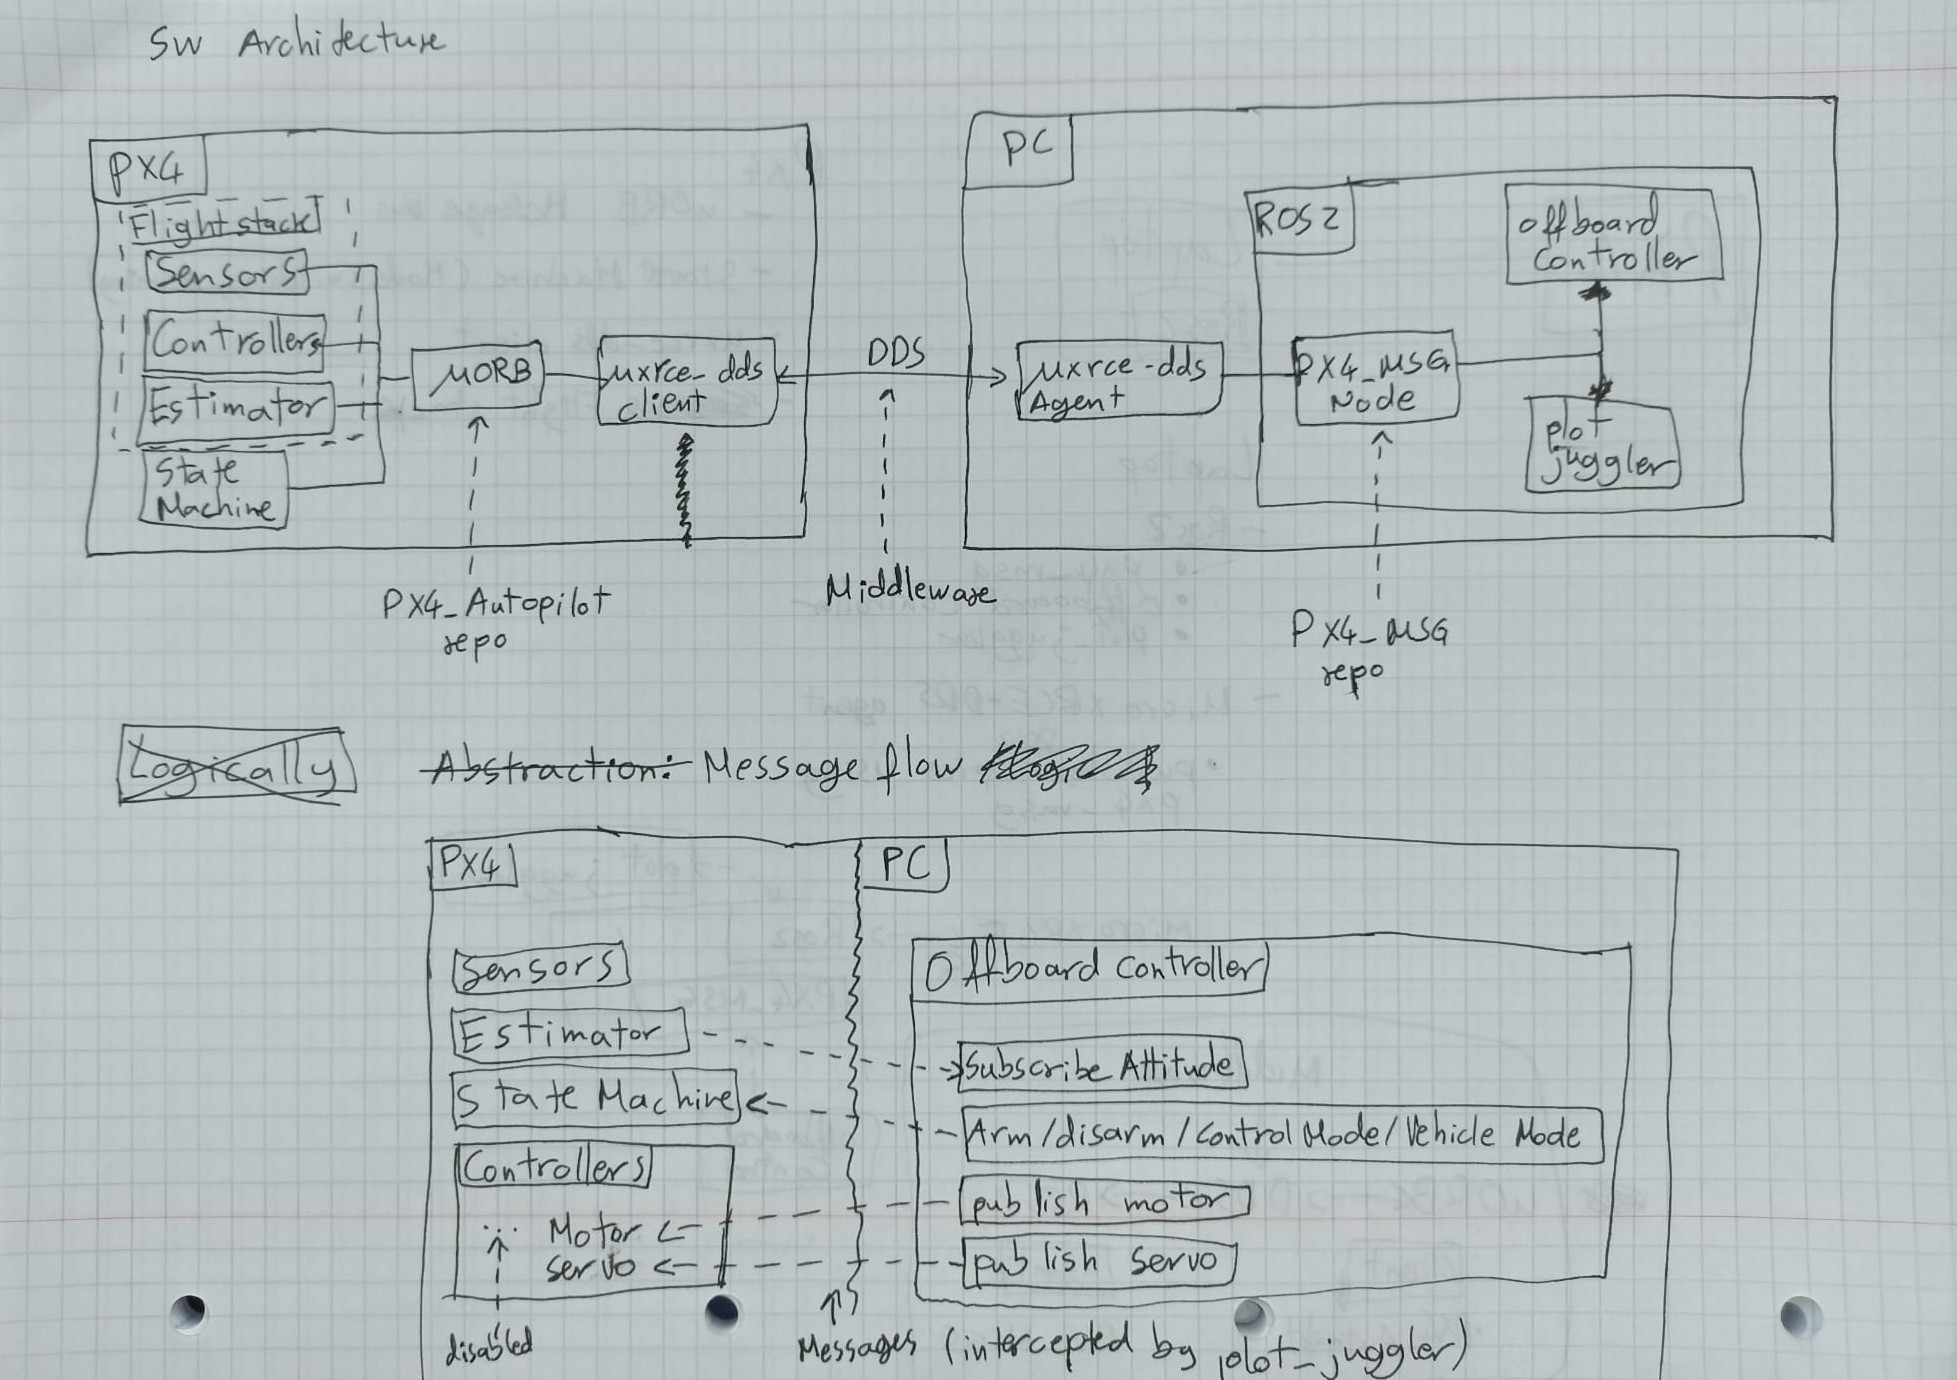
\includegraphics[width=0.9\textwidth]{imgs/Software Diagram.jpg}
    \caption{Software Architecture}
    \label{fig:software_architecture}
\end{figure}

\begin{figure}[H]
    \centering
    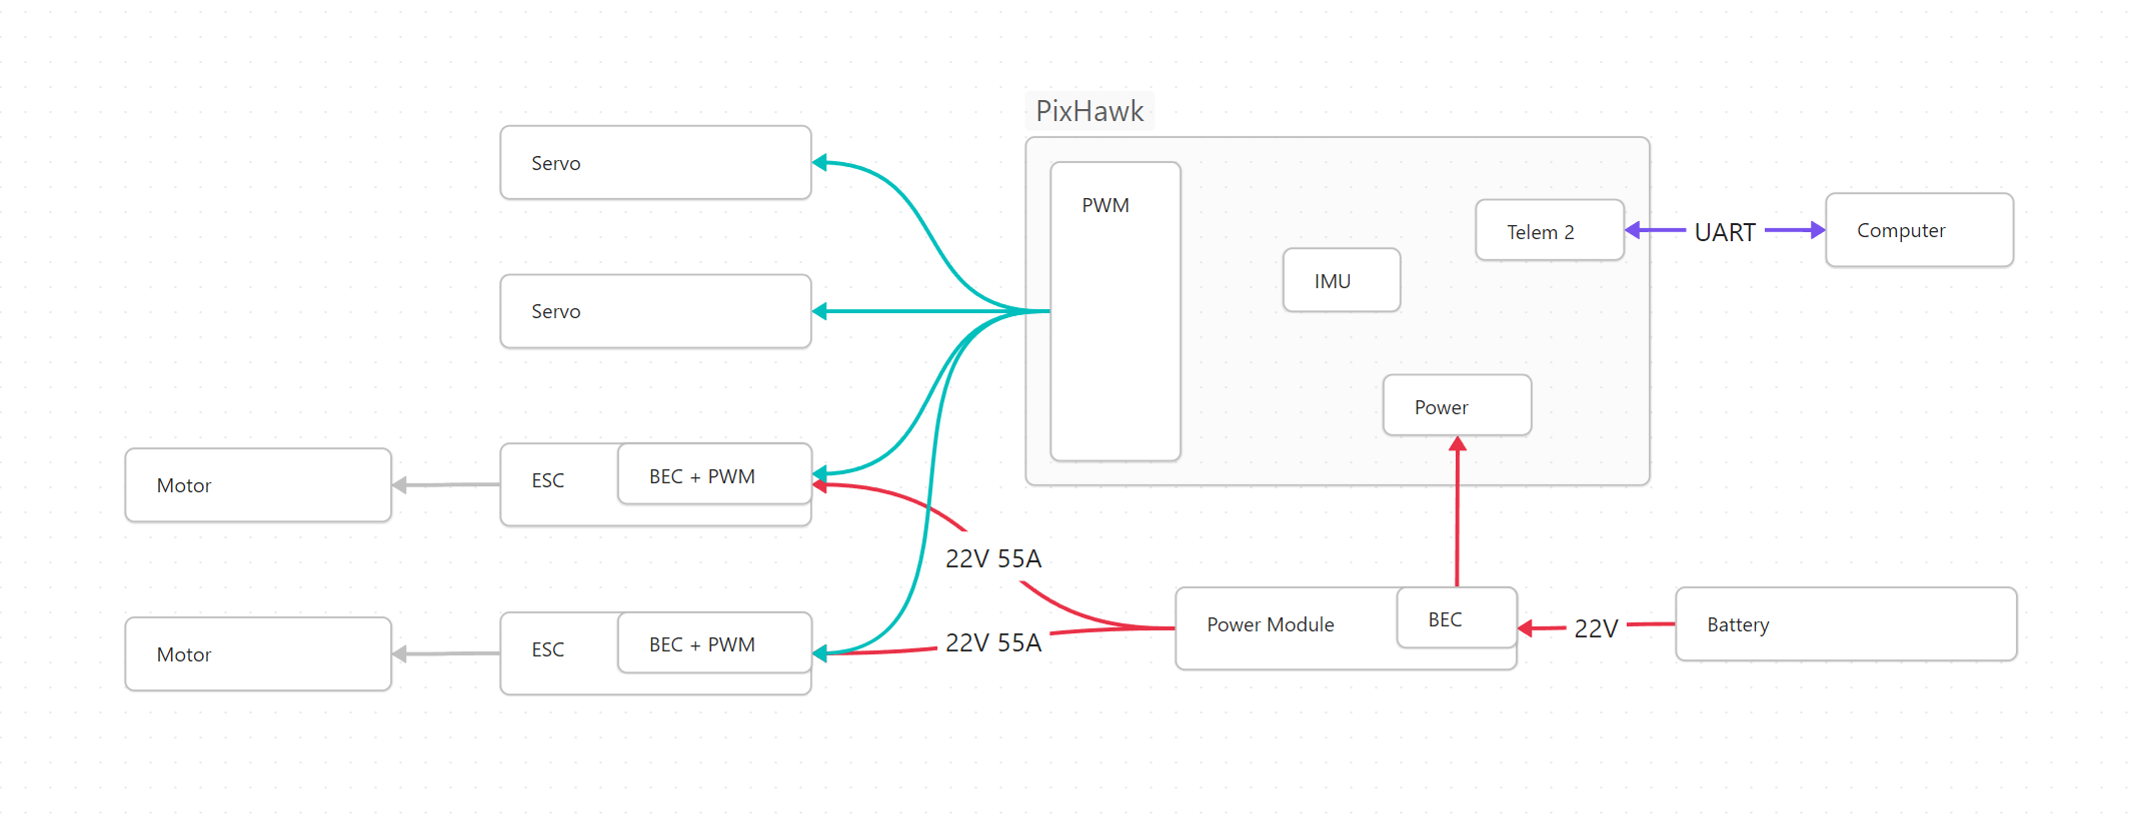
\includegraphics[width=0.9\textwidth, trim=30 30 30 30, clip]{imgs/Hardware Diagram.png}
    \caption{Hardware Block Diagram}
    \label{fig:hardware_block_diagram}
\end{figure}

The system is composed of two main components: the PX4 flight controller and the offboard computer. 
The PX4 flight controller is responsible for the hardware drivers, sensors readings, and position and attitude estimation. 
The offboard computer is responsible for using the sensor data to actuate the servos and motors. 

\subsection{PX4}

To enable offboard mode, PX4's internal state machine mode has to be changed to offboard (using \verb|VehicleCommand| Message).

In addition, the offboard computer has to send a heartbeat message (\verb|OffboardControlMode|) to PX4 with a frequency of, at least, 2 Hz, so that it knows that the offboard computer is connected. Additionally, it enables offboard control only after receiving the signal for more than a second, and will regain control if the signal stops, which will switch to failsafe mode, currently configured to disarm the vehicle. This behaviour is part of PX4's safety features. 
This is explain in greater detail in \url{https://docs.px4.io/main/en/flight_modes/offboard.html}. \\

To control the servos and motors, the offboard computer has to send a message (\verb|OffboardControlMode|), informing the level of the PX4 control architecture at which offboard setpoints will be injected. In this case, only direct actuation is enabled. 
Another message (\verb|VehicleControlMode|) has to be sent to disable (i.e. bypass) the default controller algorithms. In this case, all default controllers are disabled, and offboard control is enabled. 

\begin{figure}[H]
    \centering
    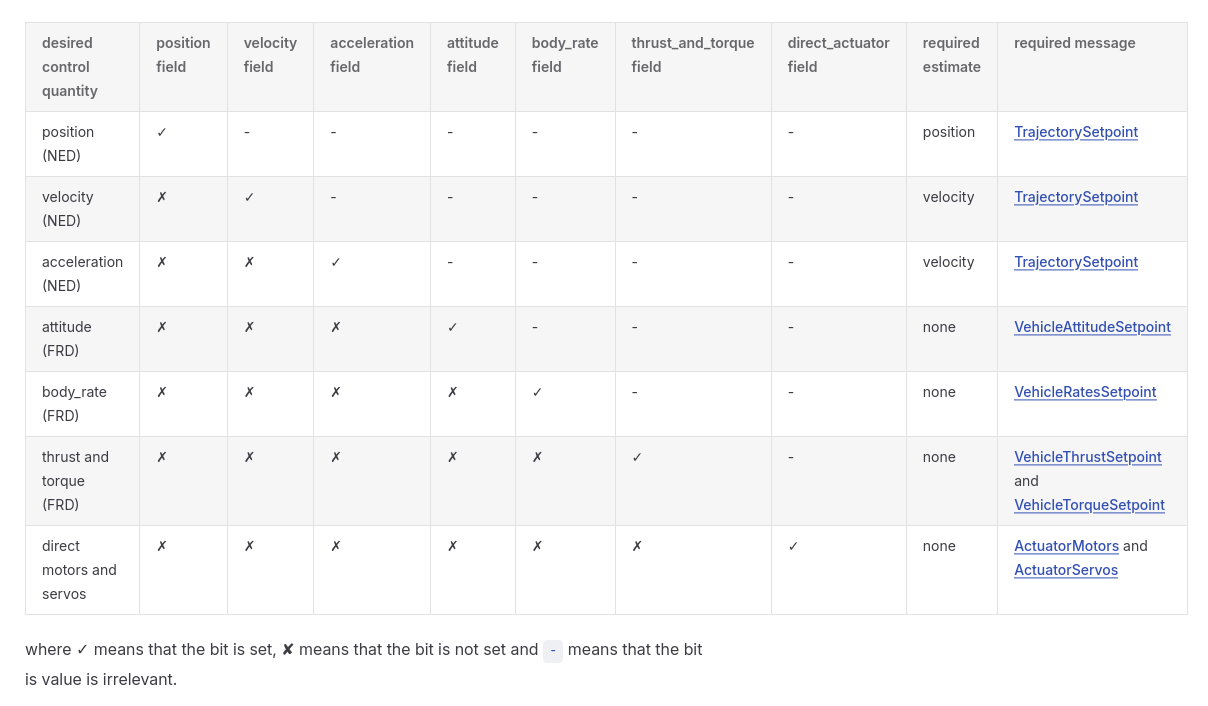
\includegraphics[width=0.8\textwidth]{imgs/OffboardControlMode authority table.png}
    \caption{OffboardControlMode Message Description}
    \label{fig:offboard_control_mode}
\end{figure}

Afterwards, the offboard computer can send the desired PWM values to the motors (\verb|ActuatorMotors|) and servos (\verb|ActuatorServos|). 
This is also explained in greater detail in \url{https://docs.px4.io/main/en/flight_modes/offboard.html#ros-2-messages}. 

Due to PX4's safety features, the motors are only enabled when the vehicle is armed\footnote{\url{https://docs.px4.io/main/en/advanced_config/prearm_arm_disarm.html\#arm-disarm-prearm-configuration}}. 
This menas that the offboard computer has to arm the vehicle (\verb|VehicleCommand|) before sending the PWM values to the motor. 

All of these messages are part of the uORB communication bus, and are mapped to ROS2 messages\footnote{\url{https://docs.px4.io/main/en/msg_docs/}}. 
The section \ref{sec::demo} describes the uORB messages used in this demo.

\subsection{uXRCE-DDS}

To connect PX4 to ROS2, PX4 uses uXRCE-DDS, which is a lightweight implementation of DDS. 
This acts as a middleware between the uORB, used between modules in PX4, and the ROS2 topics, used between ROS2 nodes. 
To use uXRCE-DDS, a uXRCE-DDS client runs in PX4, and a uXRCE-DDS agent runs in the offboard computer. 
This is shown in the diagram below: 

\begin{figure}[H]
    \centering
    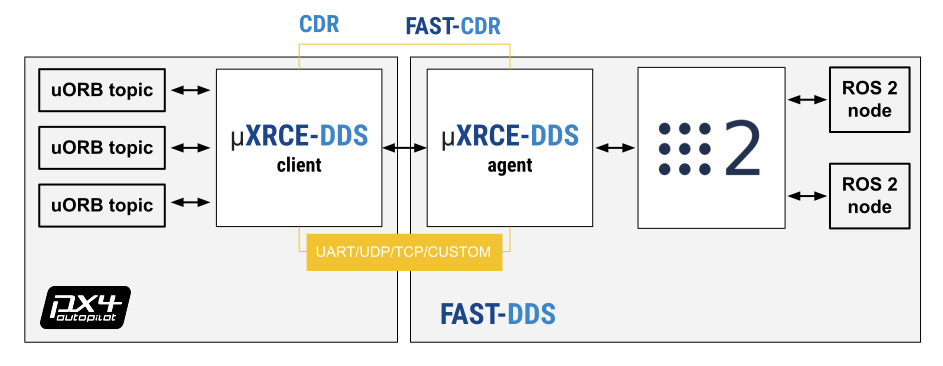
\includegraphics[width=0.8\textwidth]{imgs/architecture_xrce_dds_ros2.png}
    \caption{Software architecture connecting PX4 to ROS2 using uXRCE-DDS}
    \label{fig:architecture_xrce_dds_ros2}
\end{figure}

In our case, the connection between client and agent is done using a serial connection. 
This is also explained in greater detail in \url{https://docs.px4.io/main/en/middleware/uxrce_dds.html}. 

\subsection{ROS2}

The Robot Operating System (ROS) is a set of software libraries and tools for building robot applications\footnote{\url{https://www.ros.org/}}. 
ROS 2 is a middleware based on a strongly-typed, anonymous publish/subscribe mechanism that allows for message passing between different processes. 
At the heart of any ROS 2 system is the ROS graph. The ROS graph refers to the network of nodes in a ROS system and the connections between them by which they communicate. 

The offboard computer  ROS2 workspace, which is a set of packages that can be built and run together, available in \url{https://github.com/PedromcaMartins/e-rocket}. 

The demo workspace uses 3 packages: 
\begin{itemize}
    \item \verb|px4_msgs\footnote{\url{https://github.com/PX4/px4_msgs}}|: This package contains a node that connects to the uXRCE-DDS agent, and subsctibes to the PX4 uORB messages, exposing ROS2 topics that converting the PX4 messages to and from ROS2 messages.
    \item \verb|offboard_control|: This package contains the offboard control node that subscribes to the sensor messages, and publishes the servo and motor messages.
    \item \verb|plot_juggler\footnote{\url{https://plotjuggler.io/}}|: This package is used to visualize ROS2 topics and messages in real time, with the help of a GUI.
\end{itemize}



\clearpage
\section{Setup}

\subsection{PX4}

Before being able to test this demo, a number of configurations are required. 
Most of these steps follow the official PX4 documentation, and are not specific to this project, available in \url{https://docs.px4.io/main/en/dev_setup/getting_started.html}. 

\subsubsection{Firmware}

The first step when using hardware like PixHawk, which runs the PX4 software, is to flash the PX4 firmware. 
The team chose the latest stable version, version v1.15.2\footnote{\url{https://github.com/PX4/PX4-Autopilot/releases/tag/v1.15.2}}. 

\subsubsection{Airframe}

After installing firmware you need to select a vehicle type and frame configuration. 
This applies appropriate initial parameter values for the selected frame, such as the vehicle type, number of motors, relative motor position, and so on. 
The team followed the official tutorial\footnote{\url{https://docs.px4.io/main/en/config/airframe.html}}. 

The team started by using a baloon frame, because the vehicle is uncontrolled (baloon frame has disabled the native flight controller algorithms). 
This turned out to not be unfeasable, as this frame also disables the ability to configure servos, which our system requires. 
Instead, the team used the generic quadcopter frame\footnote{\url{https://docs.px4.io/main/en/airframes/airframe_reference.html\#quadrotor-x}}, with a custom generic geometry\footnote{\url{https://docs.px4.io/main/en/config/actuators.html\#geometry}}. 

The team always intends to control this system using the offboard computer. This means that the relative motor positions configured in the geometry, which are used for PX4 controller allocation don't need to be configured. Additionally, as mentioned in Section \ref{sec::background}, the PX4 existing controllers don't support the TVC mechanism, and by extension, our system. 

\subsubsection{Actuator setup}
Using a generic geometry, the 2 motors were configured to the outputs PWM AUX (FMU Board output) 3 and 4, and the 2 servos were configured to the outputs PWM MAIN (I/O Board output) 5 and 6. 

Note that for controlling motors, PWM AUX outputs are preferred over the PWM MAIN outputs (as they have lower latency)\footnote{\url{https://docs.px4.io/main/en/config/actuators.html\#actuator-outputs}}. 

% \subsubsection{Safety checks}
% TODO! Add stuff in this section :skull:
% add link https://docs.px4.io/main/en/ros/offboard_control.html#enable-rc-override

\subsubsection{uXRCE-DDS client setup}

The team followed the official tutorial\footnote{\url{https://docs.px4.io/main/en/middleware/uxrce_dds.html\#starting-the-client}}. 
\verb|TELEM2| Serial Port was the port used by the client. It uses the uart protocol configured to 115200 baud rate, 8 data bits, no parity, and 1 stop bit. 
% TODO! change uart parameters

\subsection{Offboard computer}

\subsubsection{uXRCE-DDS agent setup}

The team followed the official tutorial, and configured the agent to connect to the serial port where PixHaw was connected (\verb|/dev/ttyACM0|)\footnote{\url{https://docs.px4.io/main/en/middleware/uxrce_dds.html\#starting-the-agent}}. 

\subsubsection{ROS2 setup}

The team followed the official tutorial, installing ROS2 humble edition on Ubuntu 20.04\footnote{\url{https://docs.px4.io/main/en/ros2/user_guide.html\#installation-setup}}. 



\clearpage
\section{Demo}
\label{sec::demo}

This demo aligns the TVC mount with the vehicle's attitude, using the servos, and actuates the motors using a sinusoidal waveform out of sync (with the two motors). 
This demo is heavily inspired by the official PX4 ROS2 examples\footnote{\url{https://github.com/PX4/px4_ros_com}}. 

The following uORB messages are used in the demo: 

\begin{itemize}
    \item \verb|ActuatorMotors|\footnote{\url{https://docs.px4.io/main/en/msg_docs/ActuatorMotors.html}}: Sets PWM values of motors. 
    \item \verb|ActuatorServos|\footnote{\url{https://docs.px4.io/main/en/msg_docs/ActuatorServos.html}}: Sets PWM values of servos. 
    \item \verb|VehicleAttitude|\footnote{\url{https://docs.px4.io/main/en/msg_docs/VehicleAttitude.html}}: Gets the attitude data as a quaternion, from the attitude estimator. The attitude estimator uses the Extended Kalman Filter (EKF) present in PX4. 
    \item \verb|VehicleCommand|\footnote{\url{https://docs.px4.io/main/en/msg_docs/VehicleCommand.html}}: Sends commands to PX4, specifically Arming, Disarming, and change mode to Offboard. 
    \item \verb|VehicleControlMode|\footnote{\url{https://docs.px4.io/main/en/msg_docs/VehicleControlMode.html}}: Sets the control algoritms to be used by PX4. In this case, it disables all control algorithms, except for the offboard control. 
    \item \verb|OffboardControlMode|\footnote{\url{https://docs.px4.io/main/en/msg_docs/OffboardControlMode.html}}: Sets the control mode the offboard computer will use, specifically direct actuation. It also serves as the hearbeat message to remain in Offboard mode. 
\end{itemize}

\subsection{Demo Code}

The code consists of a ROS2 node that contains the logic of the demo. 
It includes the subscribers / publishers for the PX4 Messages, auxiliary functions and variables. 
There are two main components: the constructor and the callbacks. 
The full code can be found as part of the appendix in \ref{code::offboard_control.cpp}. 

The constructor of the ROS2 node is executed once, when the node is created (using \verb|spin| function in main). 

The code includes two main callbacks, which get called to respond to specific events. These callbacks include: 
\begin{itemize}
    \item The subscriber to the \verb|VehicleAttitude| message, that is called when a new message is received. It uses the attitude data to control the servos, and actuates the motors. 
    \item A timer callback function, called every 100ms, that changes the mode of the vehicle, arms and disarms the vehicle, and sends the heartbeat message. 
\end{itemize}

\subsubsection{Class OffboardControl}

The class called \verb|OffboardControl| which extends the \verb|Node| class, is the main class of the demo. 
It contains the variables and functions used. 

The function \verb|OffboardControl()| is the constructor of the class, which initializes the node, the publishers, subscribers subscribers, and both callbacks: the timer and the attitude subscriber.

\lstinputlisting[
  language=C++,
  firstline=18,
  firstnumber=18,
  lastline=51,
  caption=OffboardControl constructor
]{code/offboard_control.cpp}

\subsubsection{Attitude subscriber callback}

In the code, the function is implemented as an anonymous function, but for convenience, it is shown here as a normal function.

\lstinputlisting[
  language=C++,
  firstline=66,
  firstnumber=66,
  lastline=85,
  caption=Attitude subscriber callback
]{code/offboard_control.cpp}

The \verb|outer_ring_pwm_| and \verb|inner_beam_pwm_| are atomic variables that store the pwm values for the servos connected to the outer ring and inner beam, respectively. 
Atomic variables are used for they are shared between threads, and need to be accessed in a thread-safe manner. 

The servo control message accepts values in the range [-1, 1], -1 being the maximum negative position, and 1 the maximum positive\footnote{\url{https://docs.px4.io/main/en/msg_docs/ActuatorServos.html}}. 
The PWM values come from the roll and pitch angles and are mapped with a range [-45, 45] to [-1, 1], but constrained to [-1, 1]. 
This is done to ensure that the values are within the range of the servos. \\

If the vehicle is in offboard mode, the servo and motor messages are published. 

The \verb|publish_actuator_servos()| function uses the pwm values, and publishes them to the servo topic. 

The \verb|publish_actuator_motors()| function uses a sinusoidal wave to send two sinusoidal curves out of phase to the motors. 

\subsubsection{State Machine / Timer callback}

This function is responsible for armind, desarming, and changing the modes of the PX4 flight controller, acting as the offboard computer's state machine. 

The offboard control message serves as the heartbeat message. It has to be sent with a frequency of at least 2 Hz, otherwise PX4 will switch to the set failsafe mode\footnote{\url{https://docs.px4.io/main/en/flight_modes/offboard.html}}. 

\lstinputlisting[
    language=C++,
    firstline=88,
    firstnumber=88,
    lastline=130,
    caption=State machine / Timer callback
]{code/offboard_control.cpp}

The variable \verb|timer_callback_iteration_| is used to count the number of iterations of the timer callback. 
It also controls the duration of the demo. 

The function \verb|RCLCPP_INFO| is used to log messages to the console.

\subsubsection{OffboardControlMode Message}

The message \verb|OffboardControlMode|\footnote{\url{https://docs.px4.io/main/en/msg_docs/OffboardControlMode.html}} is used to set the control mode of the vehicle. 
It is sent with the following values: 

\lstinputlisting[
    language=C++,
    firstline=206,
    firstnumber=206,
    lastline=215,
    caption=OffboardControlMode message
]{code/offboard_control.cpp}

The values were chosen according to the table in \url{https://docs.px4.io/main/en/flight_modes/offboard.html\#ros-2-messages}.

\subsubsection{VehicleCommand Message}

The message \verb|VehicleControlMode|\footnote{\url{https://docs.px4.io/main/en/msg_docs/VehicleControlMode.html}} is used to set the control mode of the vehicle.
It is sent with the following values:

\lstinputlisting[
    language=C++,
    firstline=224,
    firstnumber=224,
    lastline=245,
    caption=VehicleControlMode message
]{code/offboard_control.cpp}

Since all control is done by the offboard computer, all control modes are disabled, except for the offboard control. 

\subsubsection{Summary}

In summary, the demo code consists of a ROS2 node that interacts with PX4 through various messages. The timer callback functions as a state machine, sending heartbeat messages and managing the vehicle's mode and arm status according to a predefined sequence. The attitude subscriber captures the vehicle's orientation from sensor data, processes it, and uses it to control servo positions and motor speeds when in offboard mode.

The main components work together in the following sequence:

\begin{enumerate}
    \item The main function initializes the ROS2 node and creates an instance of the \verb|OffboardControl| class, initializing all publishers and subscribers. 
    \item The timer callback continuously sends heartbeat messages every 100ms. 
    \item After 15 iterations (1.5 seconds), the vehicle is switched to offboard mode and armed. 
    \item While armed, the attitude subscriber processes sensor data and controls the servos and motors in real-time. 
    \item After 300 iterations (30 seconds), the vehicle is disarmed and returned to manual mode. 
\end{enumerate}

This architecture is capable of demonstrating that an offboard computer can successfully read PX4 sensor data and control actuators, fulfilling the demo's objectives.



\clearpage
\section{Results}

The demo was successfully executed. One execution of the demo was recorded and is available in \url{https://www.youtube.com/shorts/j01qkGAldi8}. 

\subsection{Attitude}

\begin{figure}[H]
    \centering
    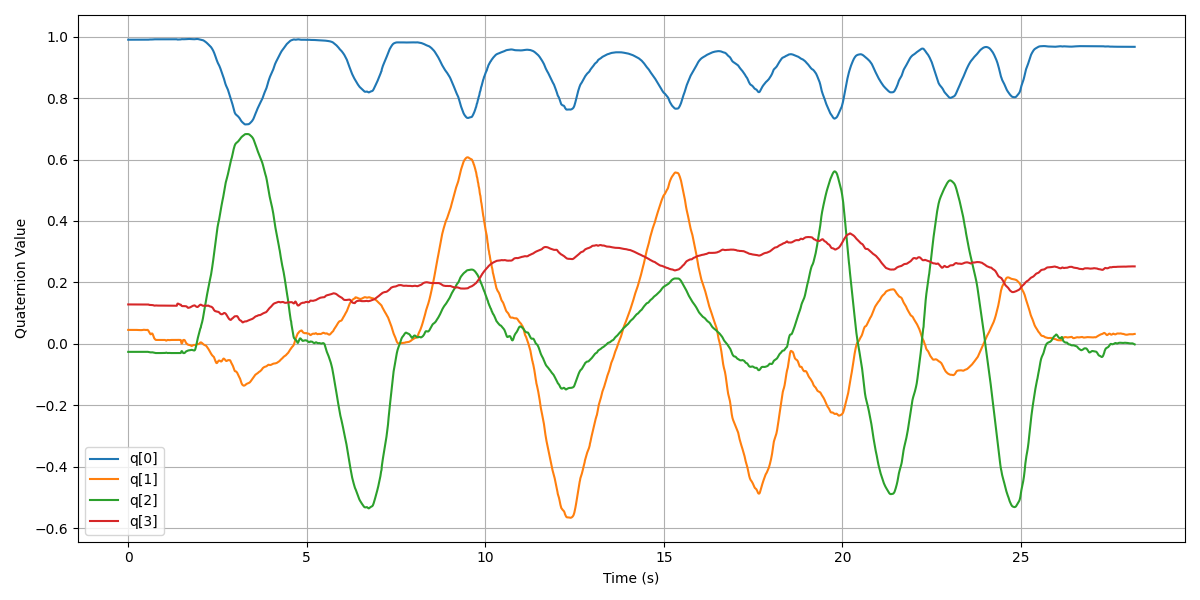
\includegraphics[width=0.8\textwidth]{imgs/demo_data/quaternion.png}
    \caption{Quaternion Components Over Time}
    \label{fig:demo_quaternion}
\end{figure}

As we can see, the quaternion values show the change in attitude of the vehicle. 

The following figures show plots from the same demo. 

\subsection{Motors}

\begin{figure}[H]
    \centering
    \label{fig:demo_motor_pwm}
    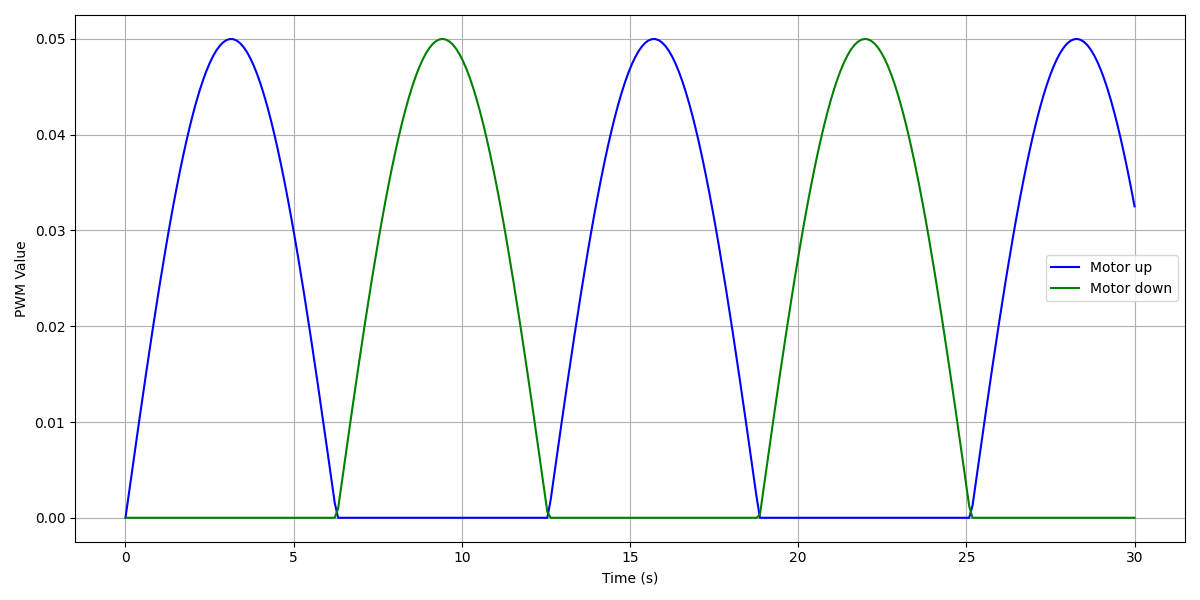
\includegraphics[width=0.8\textwidth]{imgs/demo_data/motor_pwm.png}
    \\
    \subfigure[][]{%
        \label{fig:upper_motor}%
        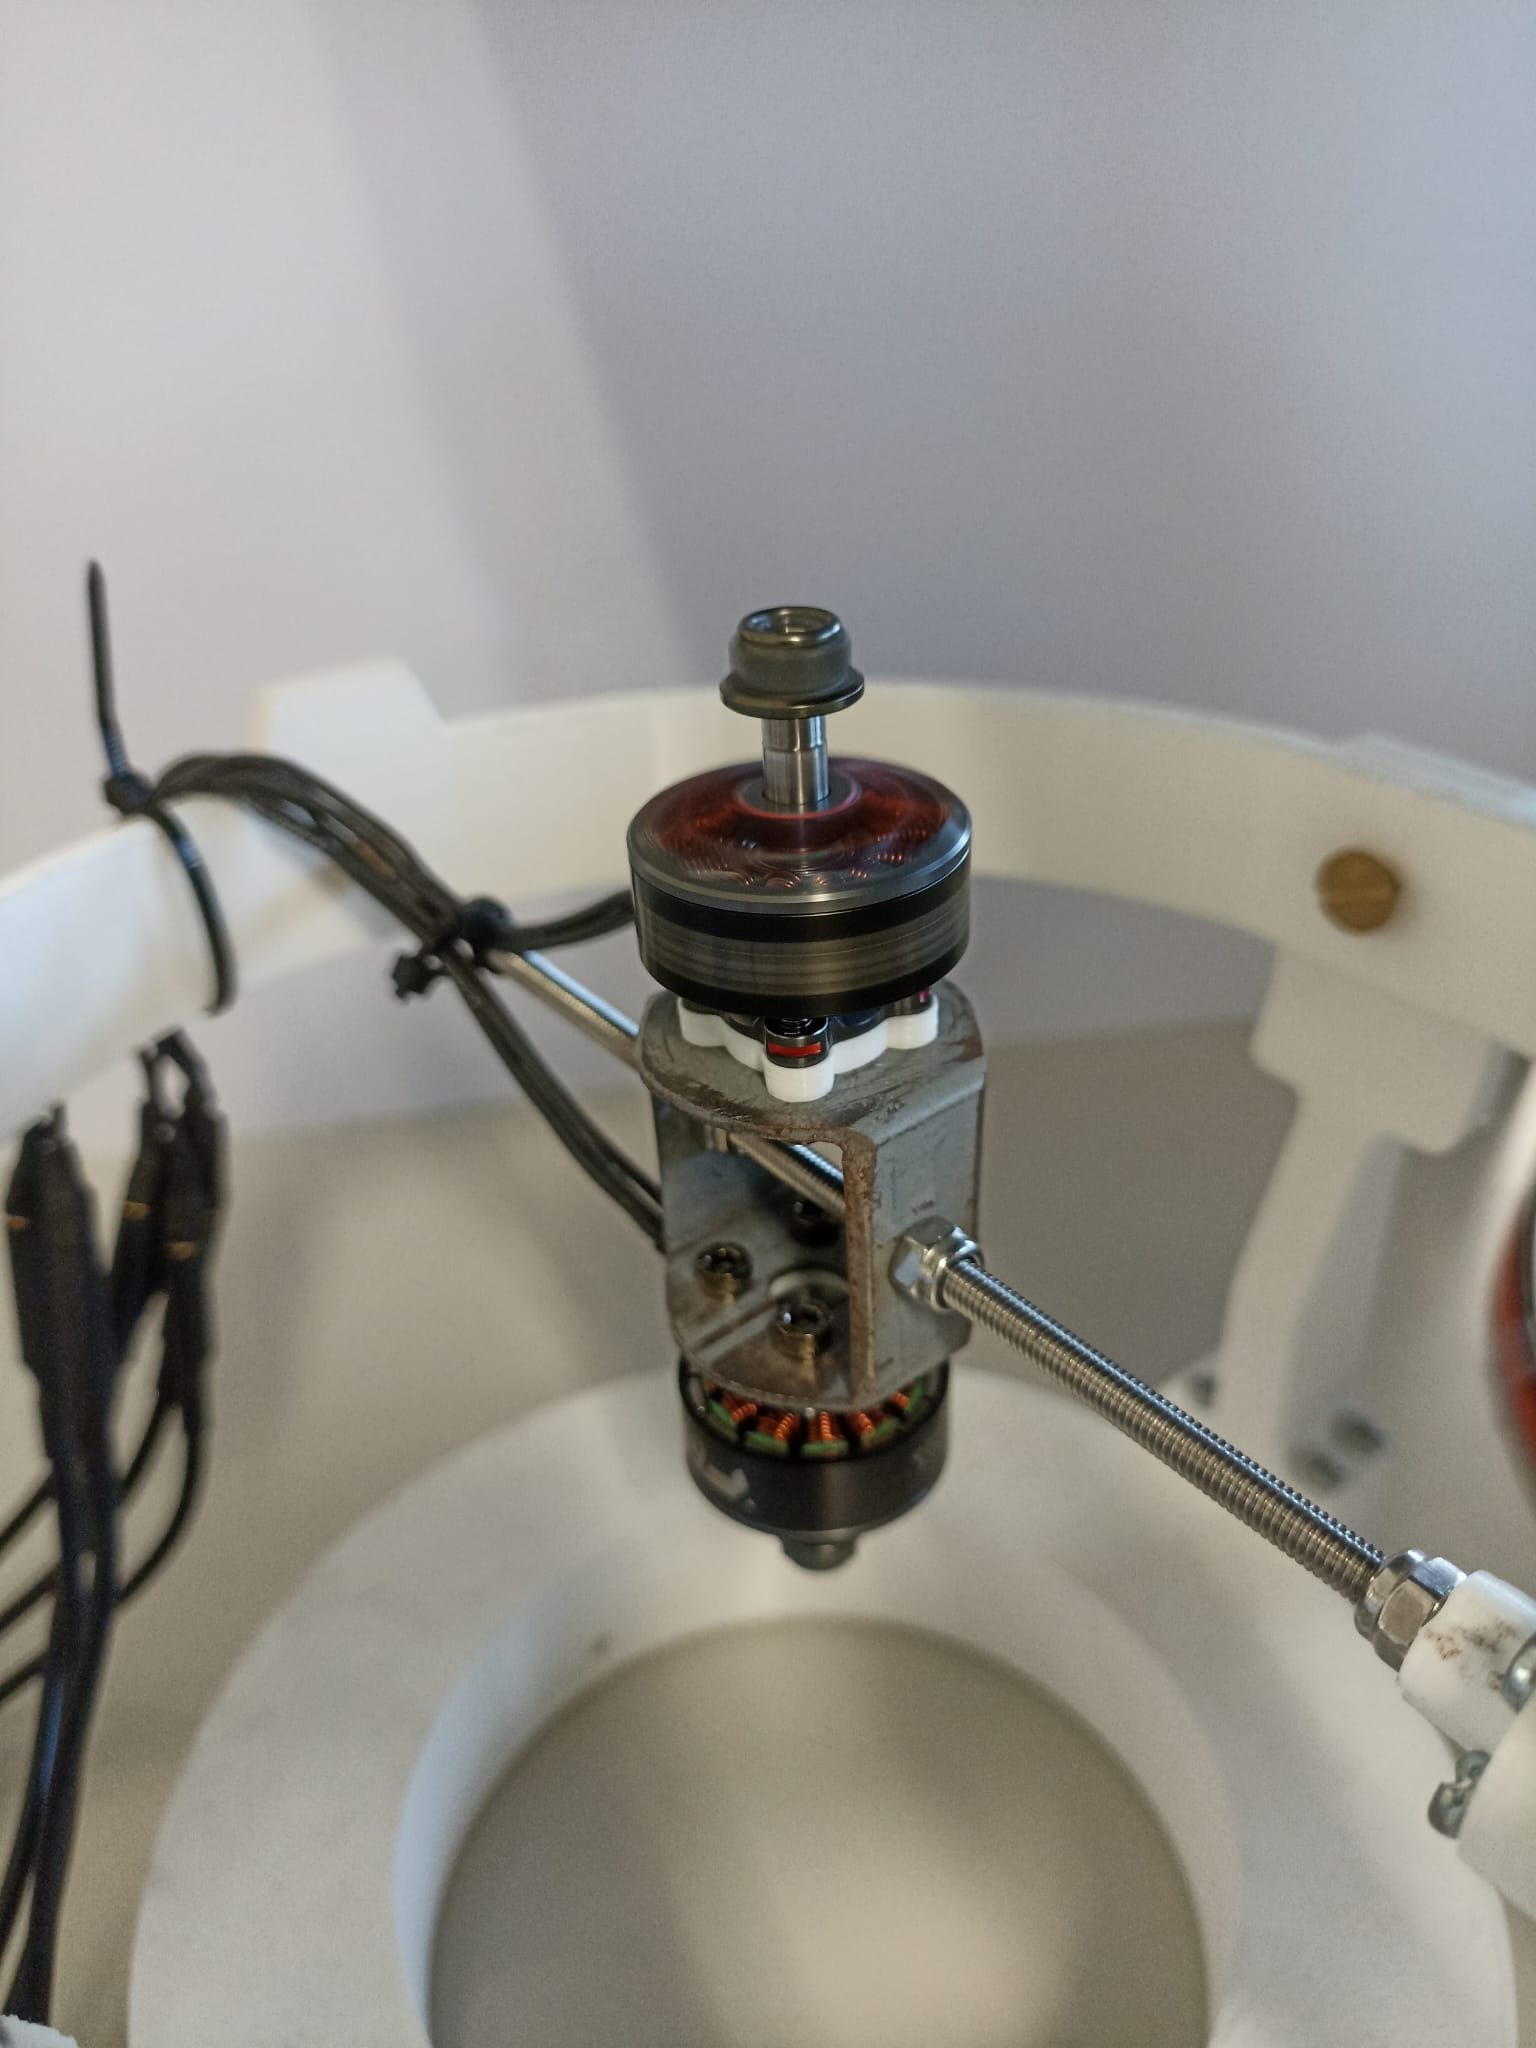
\includegraphics[width=0.23\textwidth]{imgs/demo_tvc/upper motor.jpg}
    }%
    \hspace{3pt}%
    \subfigure[][]{%
        \label{fig:bottom_motor}%
        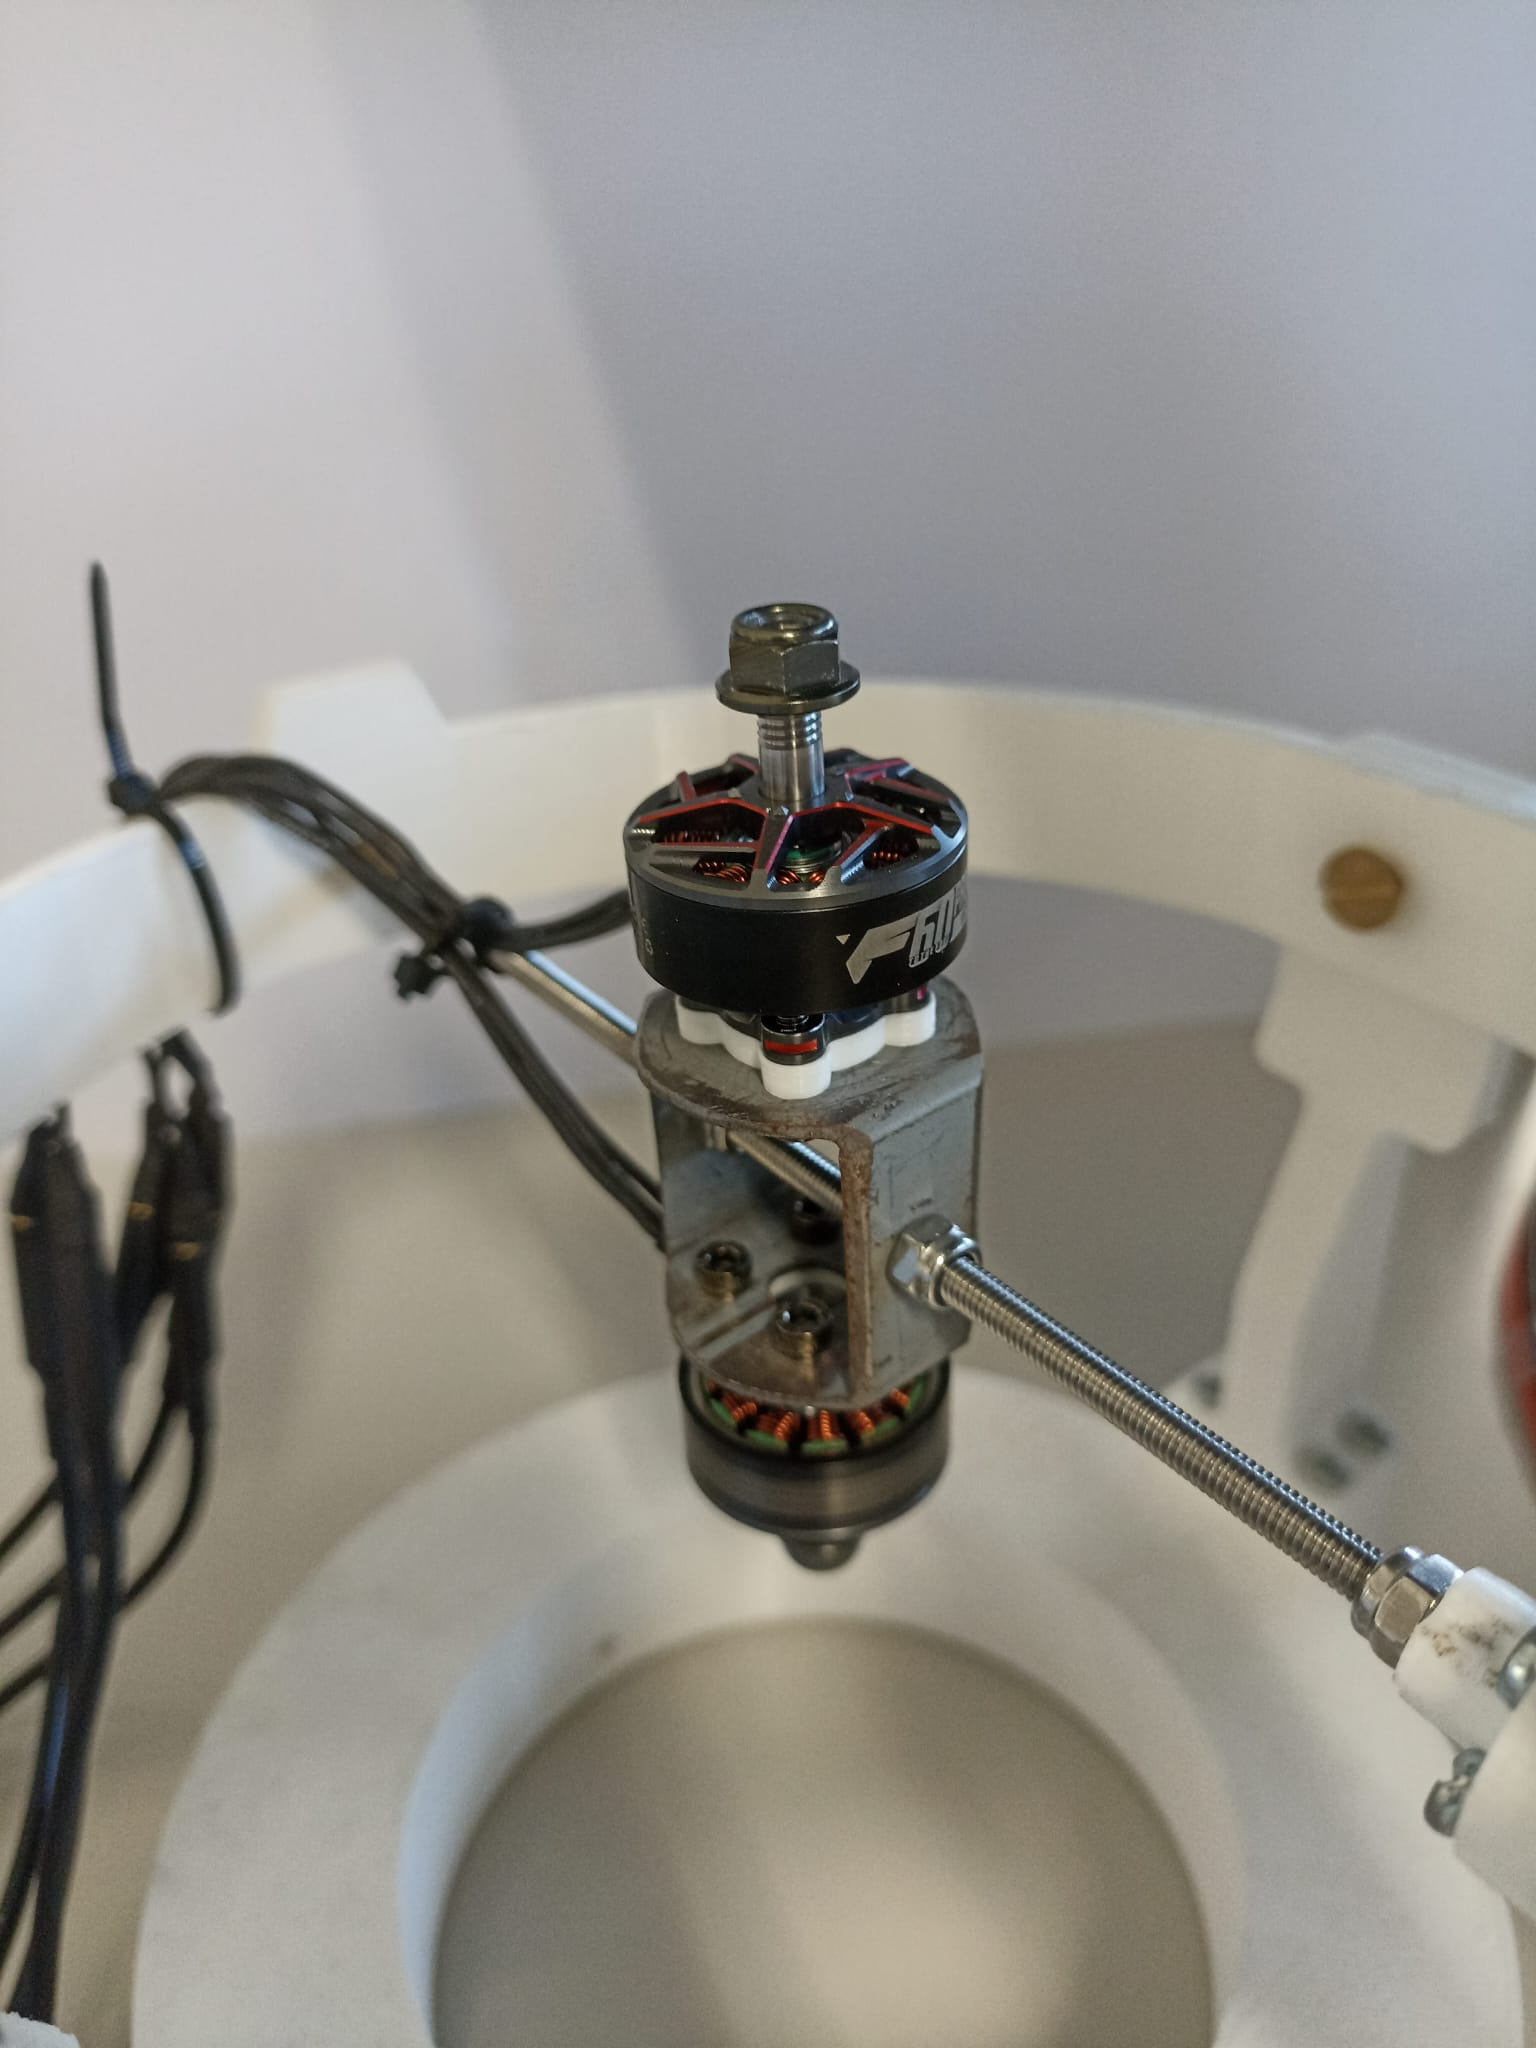
\includegraphics[width=0.23\textwidth]{imgs/demo_tvc/bottom motor.jpg}
    }
    \caption{Upper and Bottom motors spinning independently, following the sinusoidal waveform}
\end{figure}

This validates that the motors are spinning independently, and following the sinusoidal waveform.

\subsection{Servos}

\begin{figure}[H]
    \centering
    \label{fig:demo_servo_pwm}
    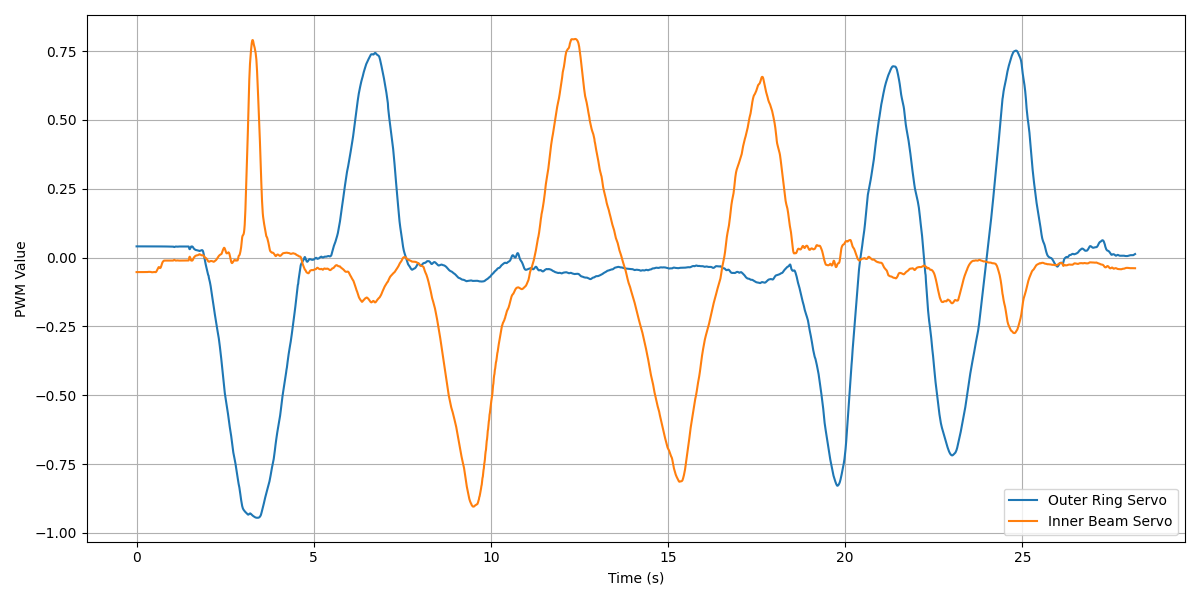
\includegraphics[width=0.8\textwidth]{imgs/demo_data/servo_pwm.png}
    \\
    \subfigure[][]{%
        \label{fig:outer_ring_left}%
        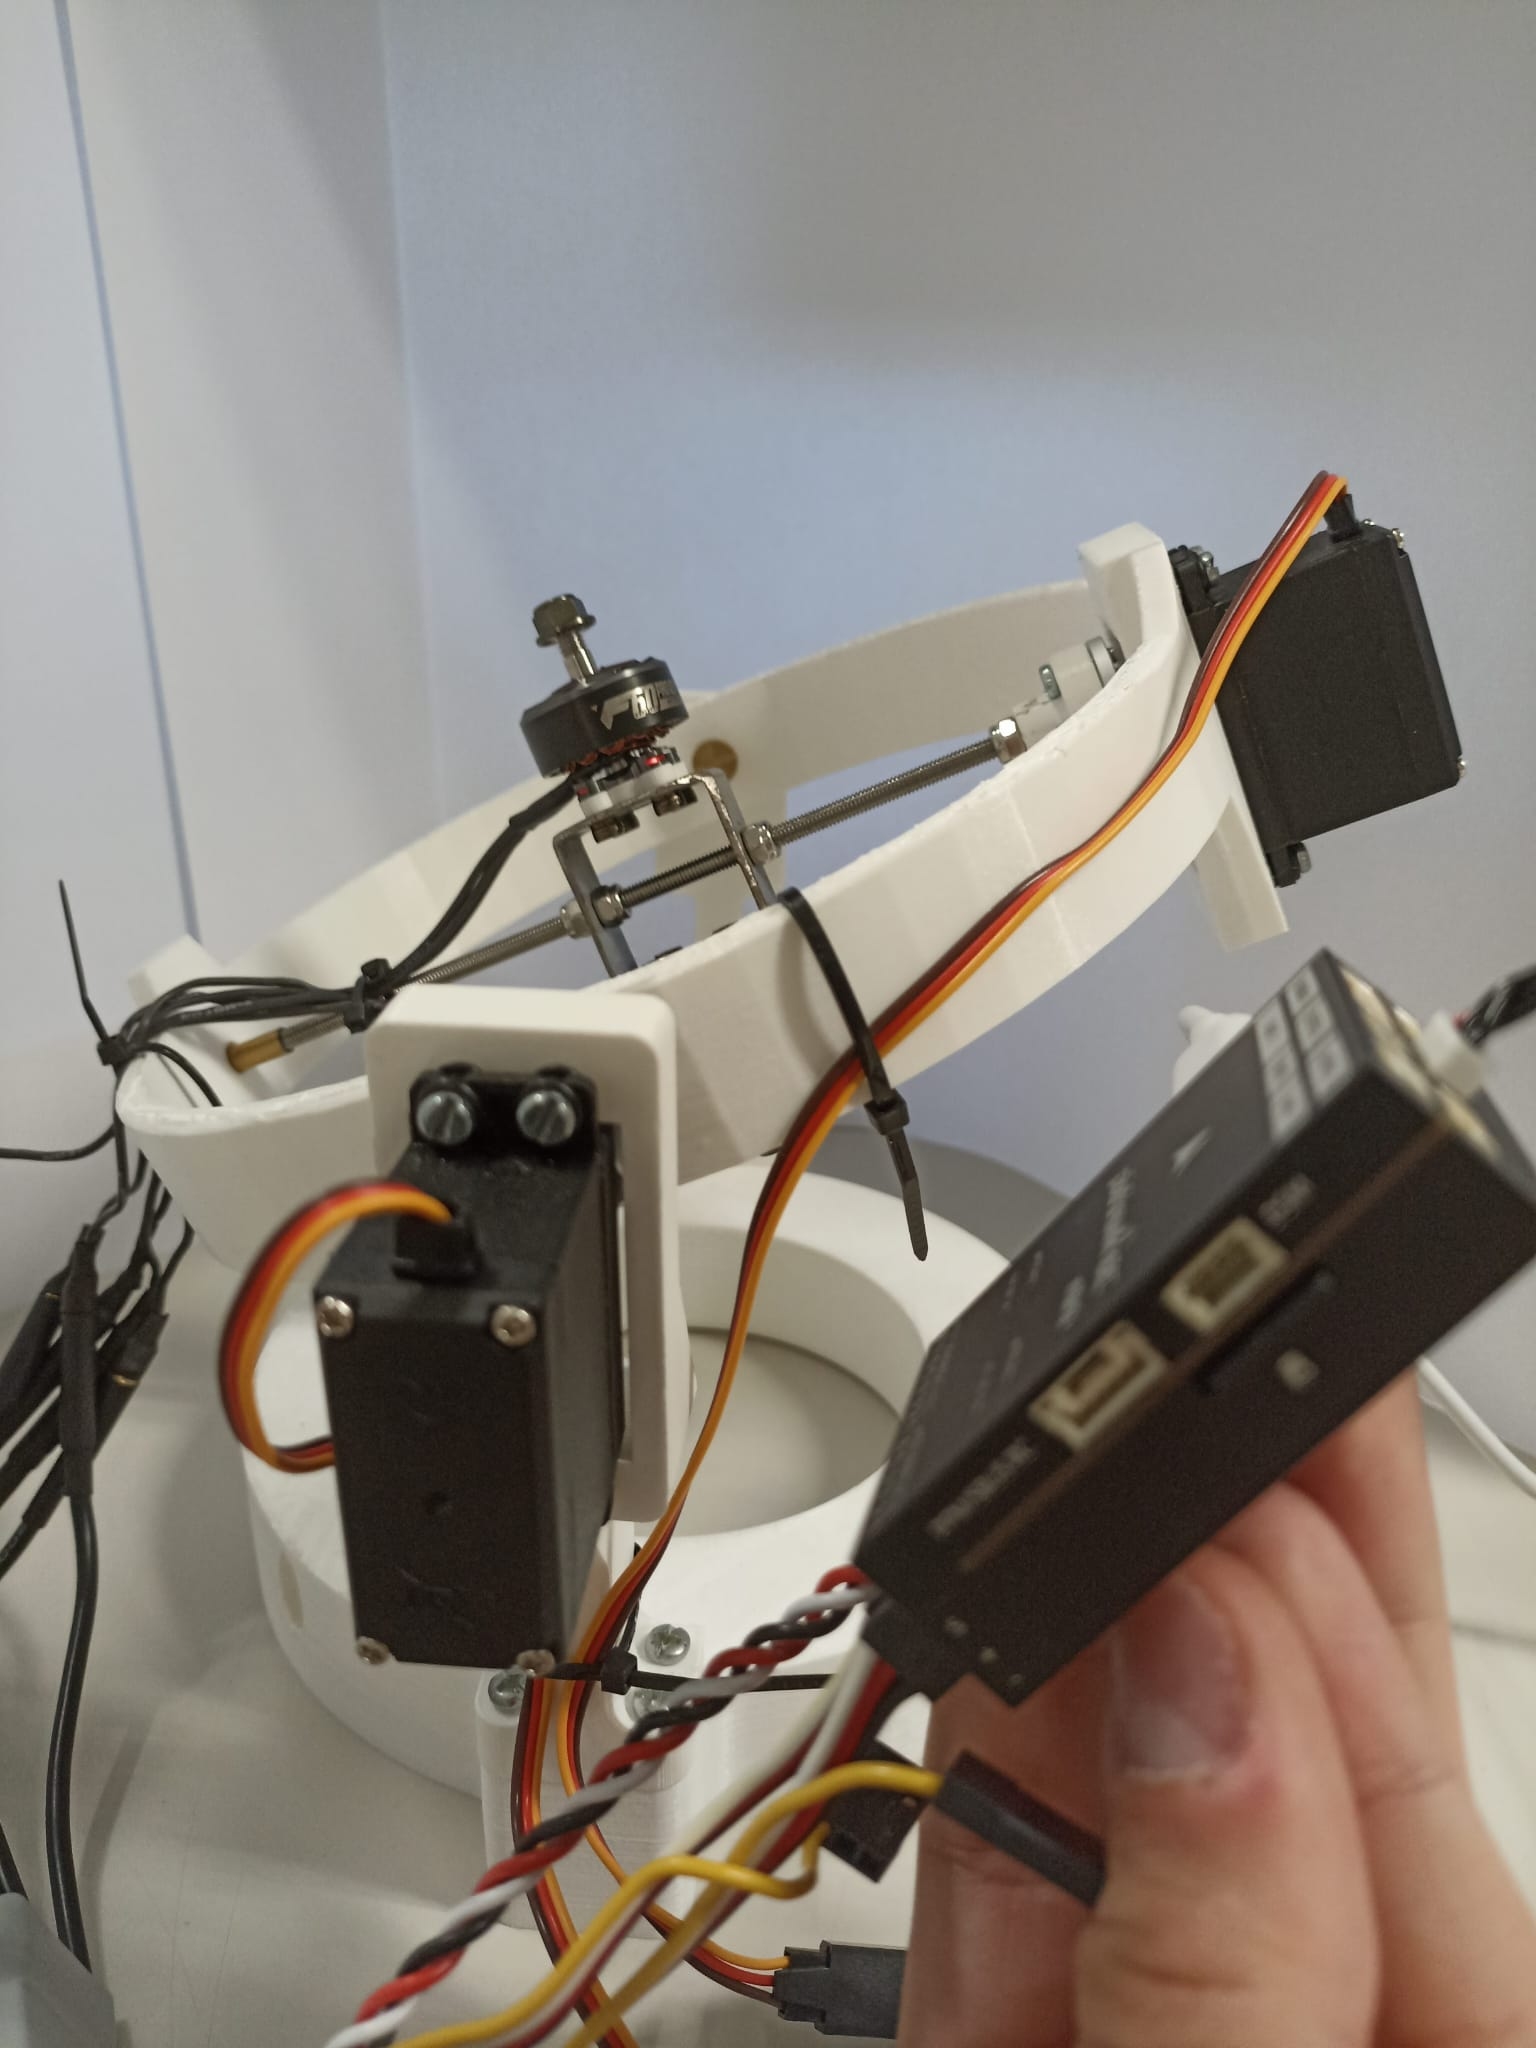
\includegraphics[width=0.23\textwidth]{imgs/demo_tvc/outer_ring_left.jpg}
    }%
    \hspace{3pt}%
    \subfigure[][]{%
        \label{fig:outer_ring_right}%
        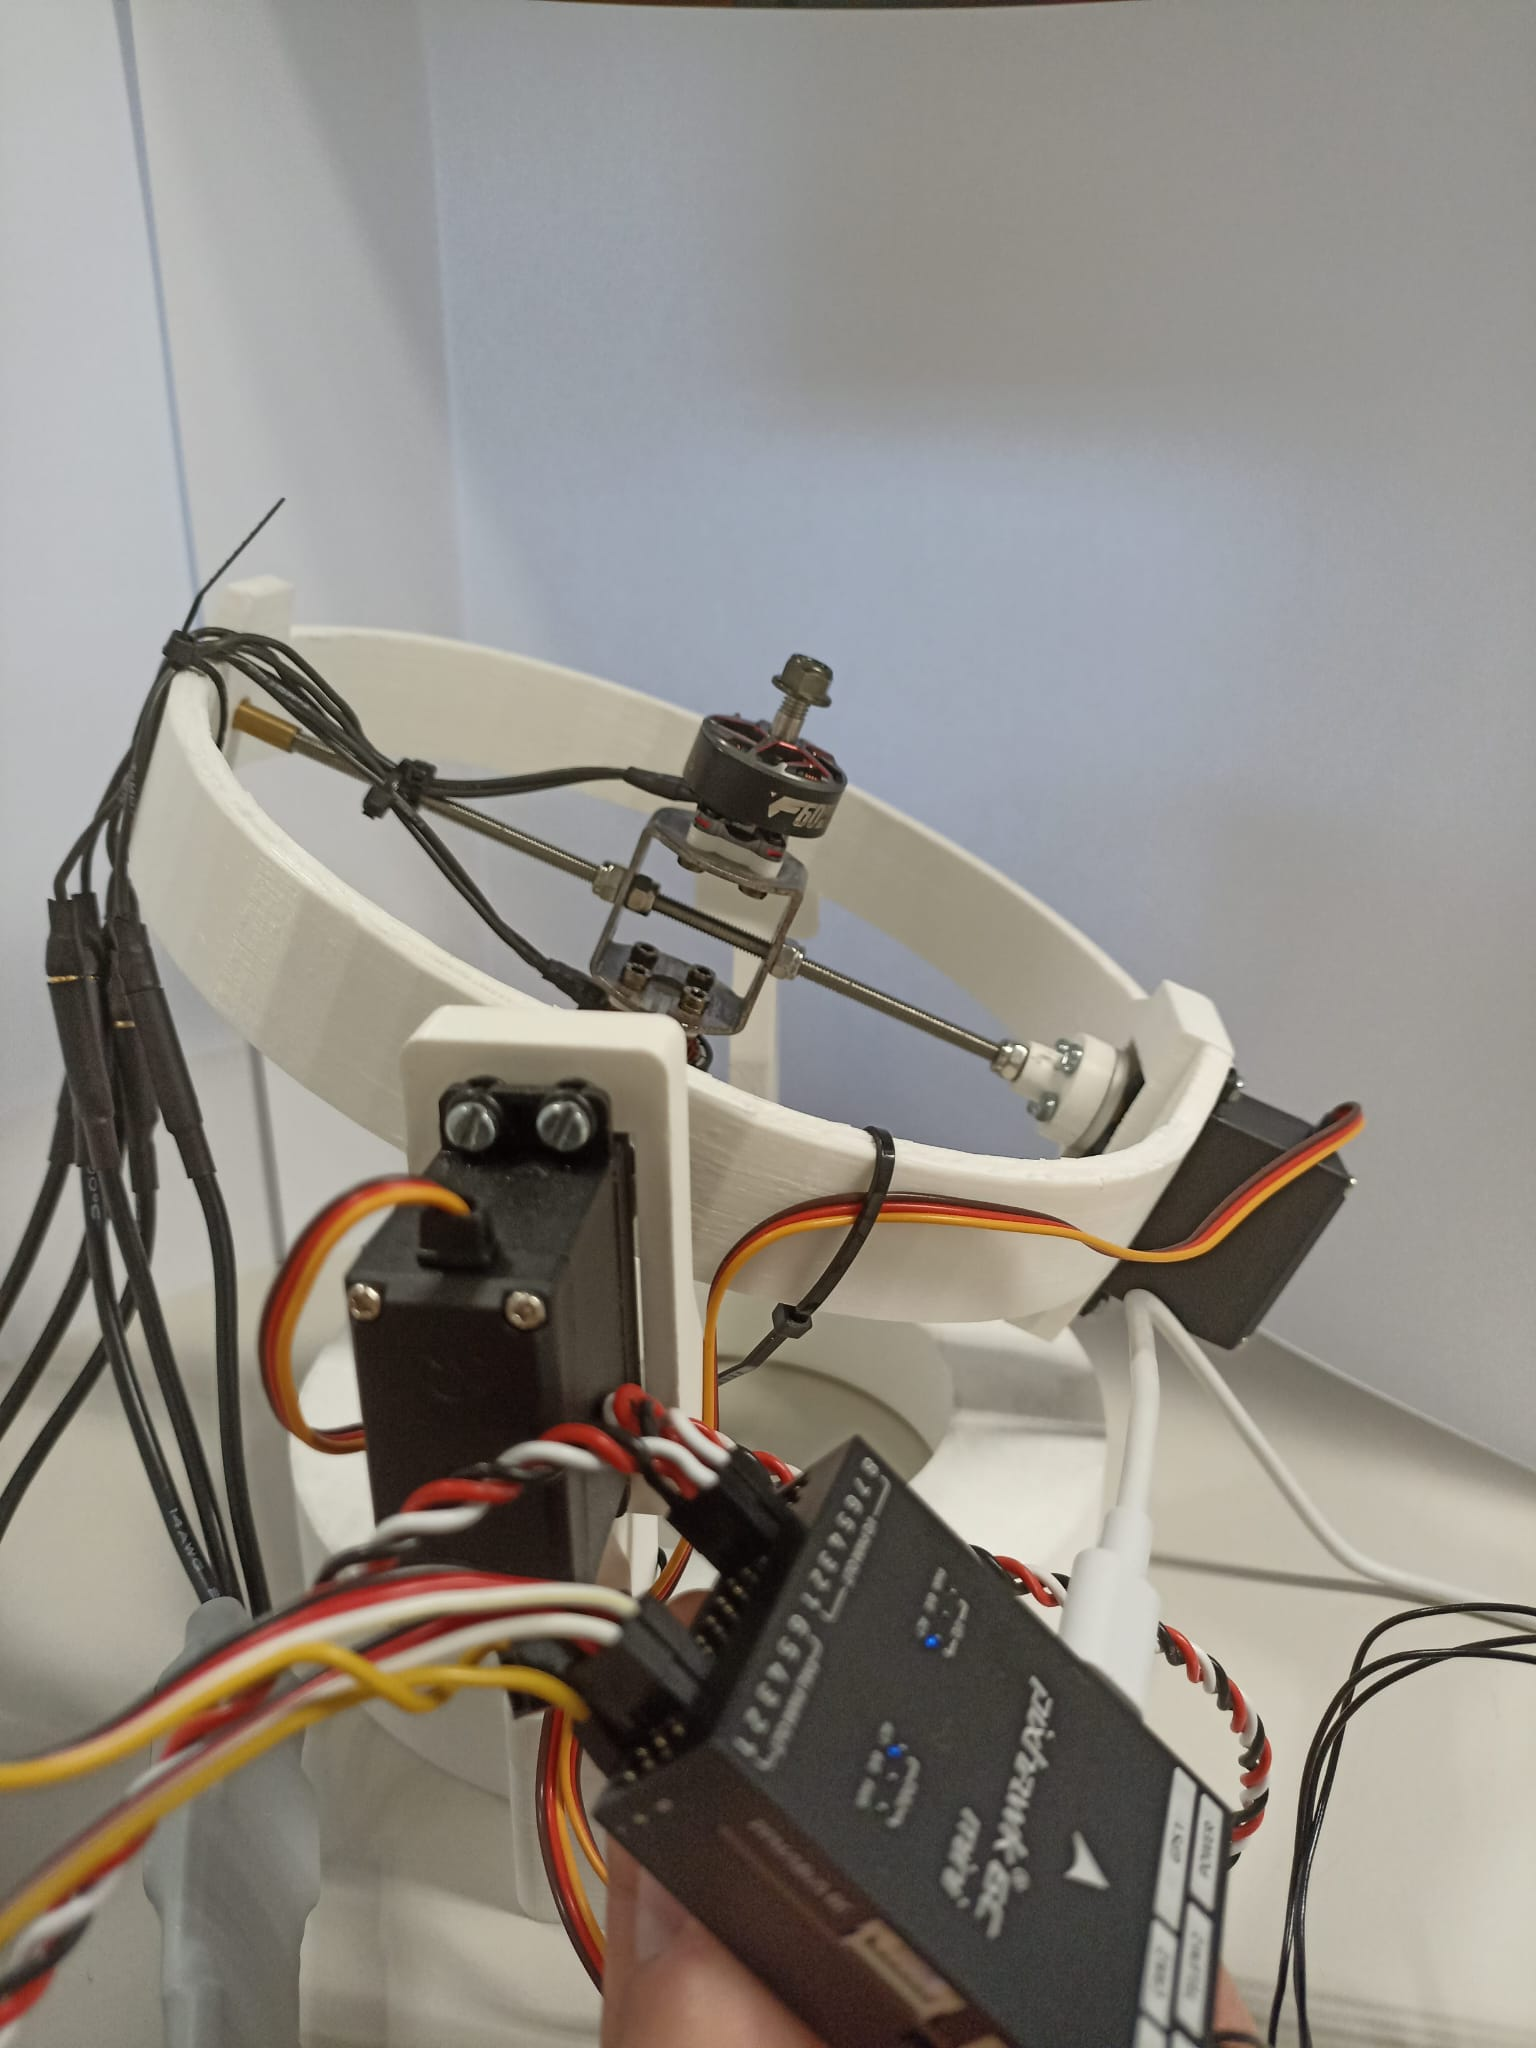
\includegraphics[width=0.23\textwidth]{imgs/demo_tvc/outer_ring_right.jpg}
    }
    \subfigure[][]{%
        \label{fig:inner_beam_left}%
        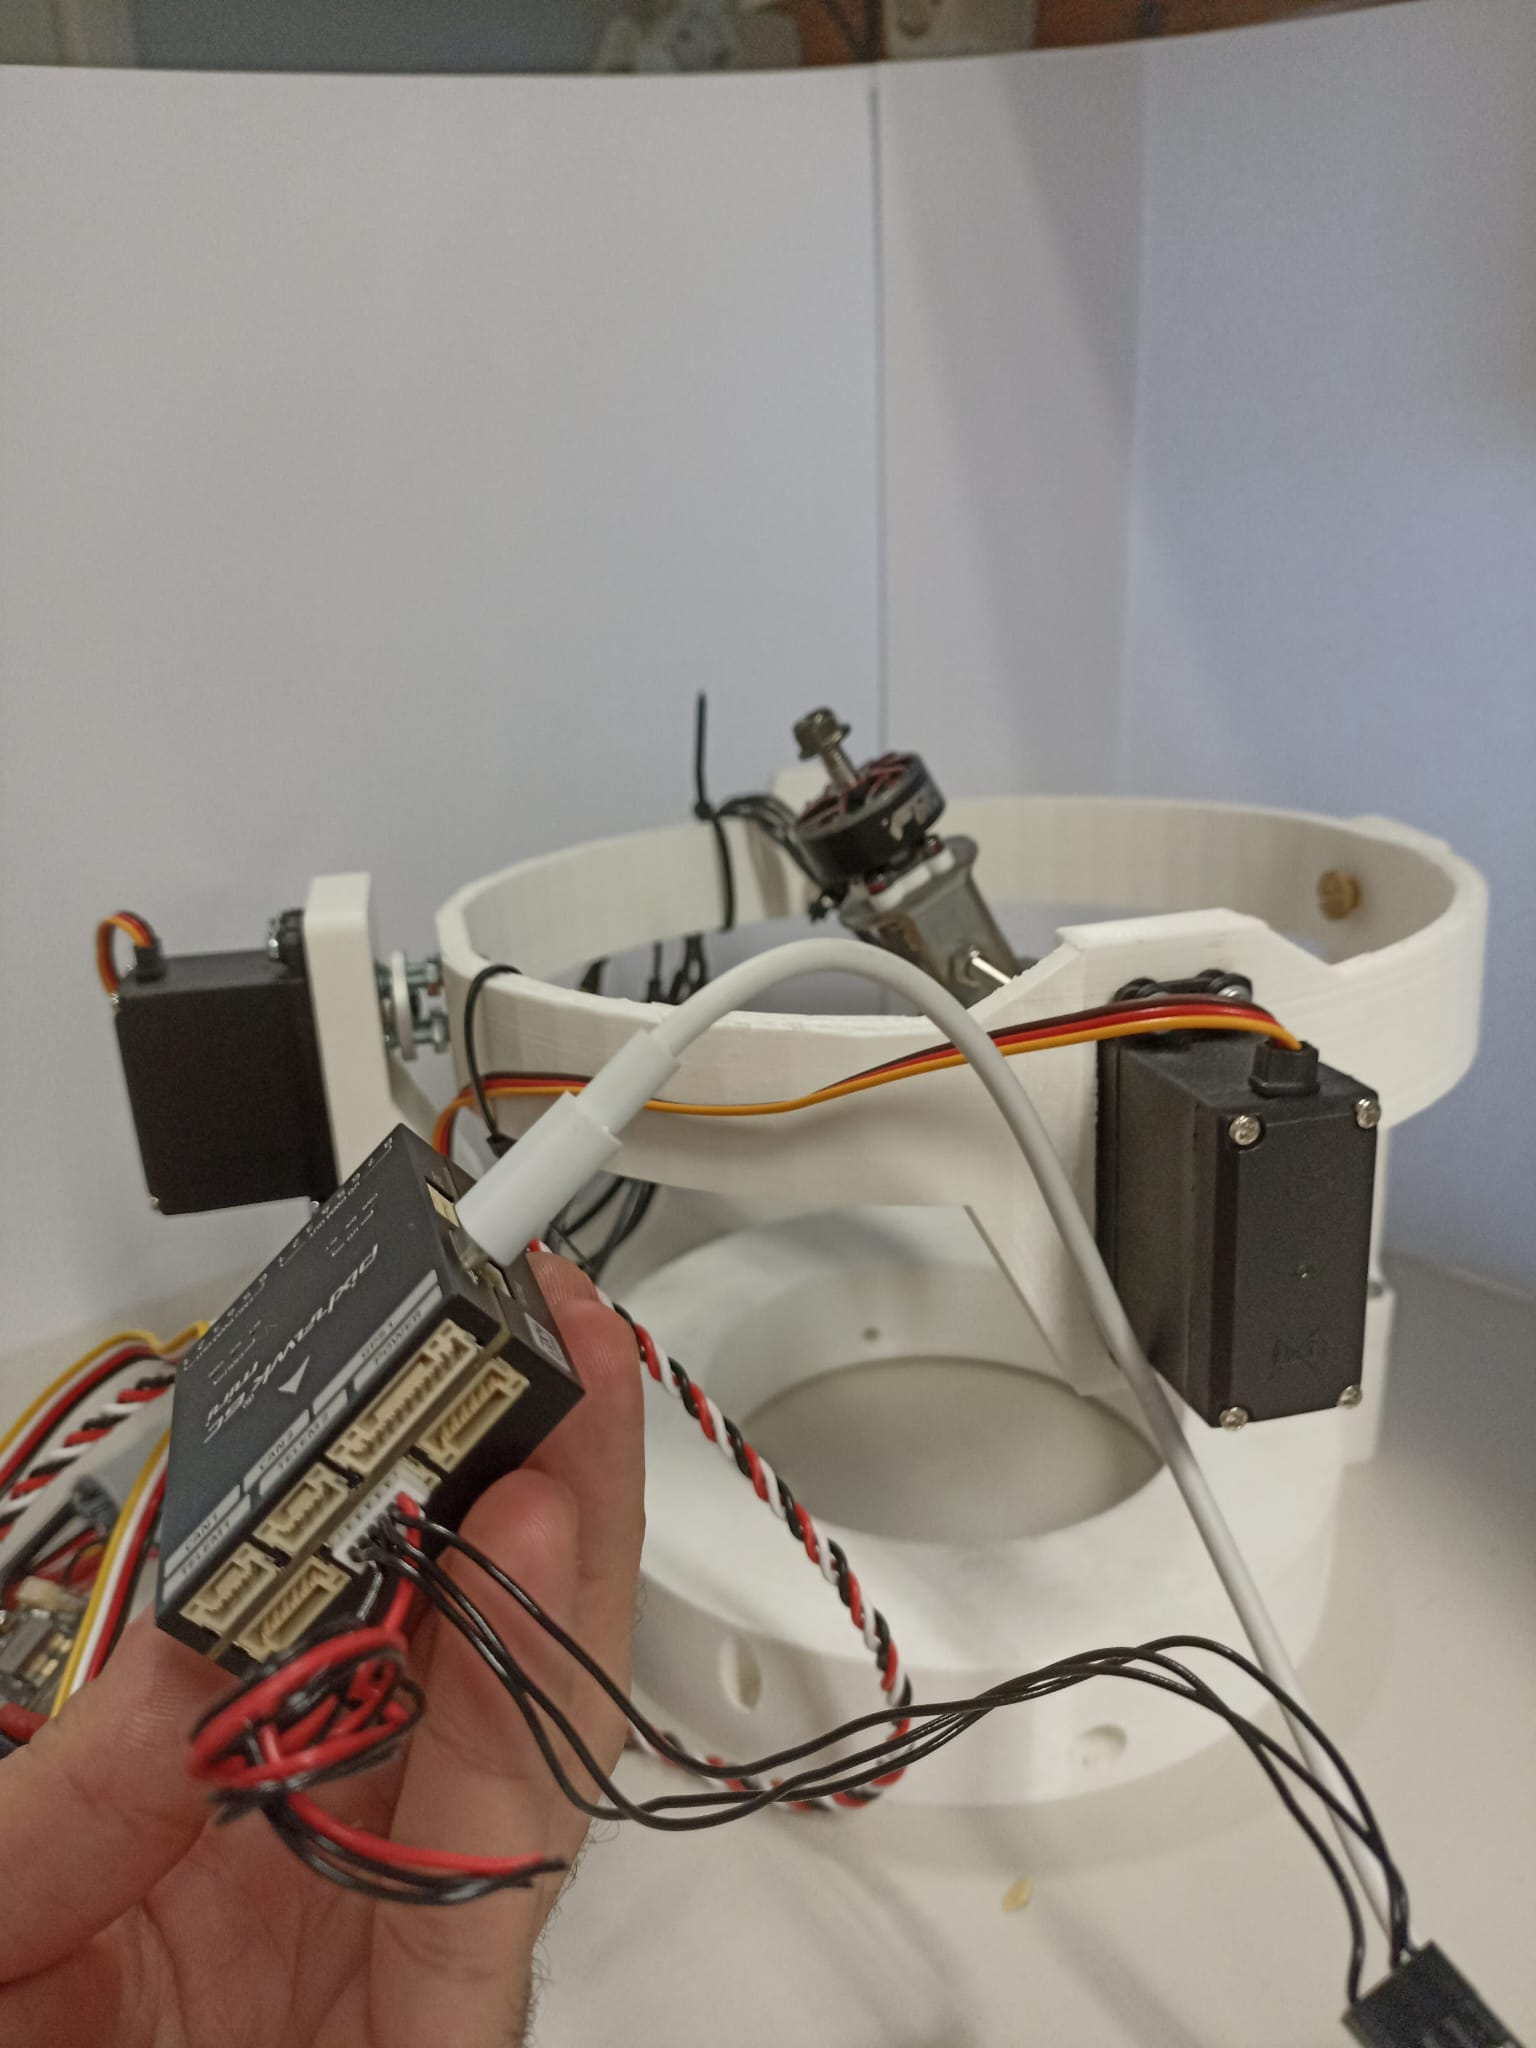
\includegraphics[width=0.23\textwidth]{imgs/demo_tvc/inner_beam_left.jpg}
    }%
    \hspace{3pt}%
    \subfigure[][]{%
        \label{fig:inner_beam_right}%
        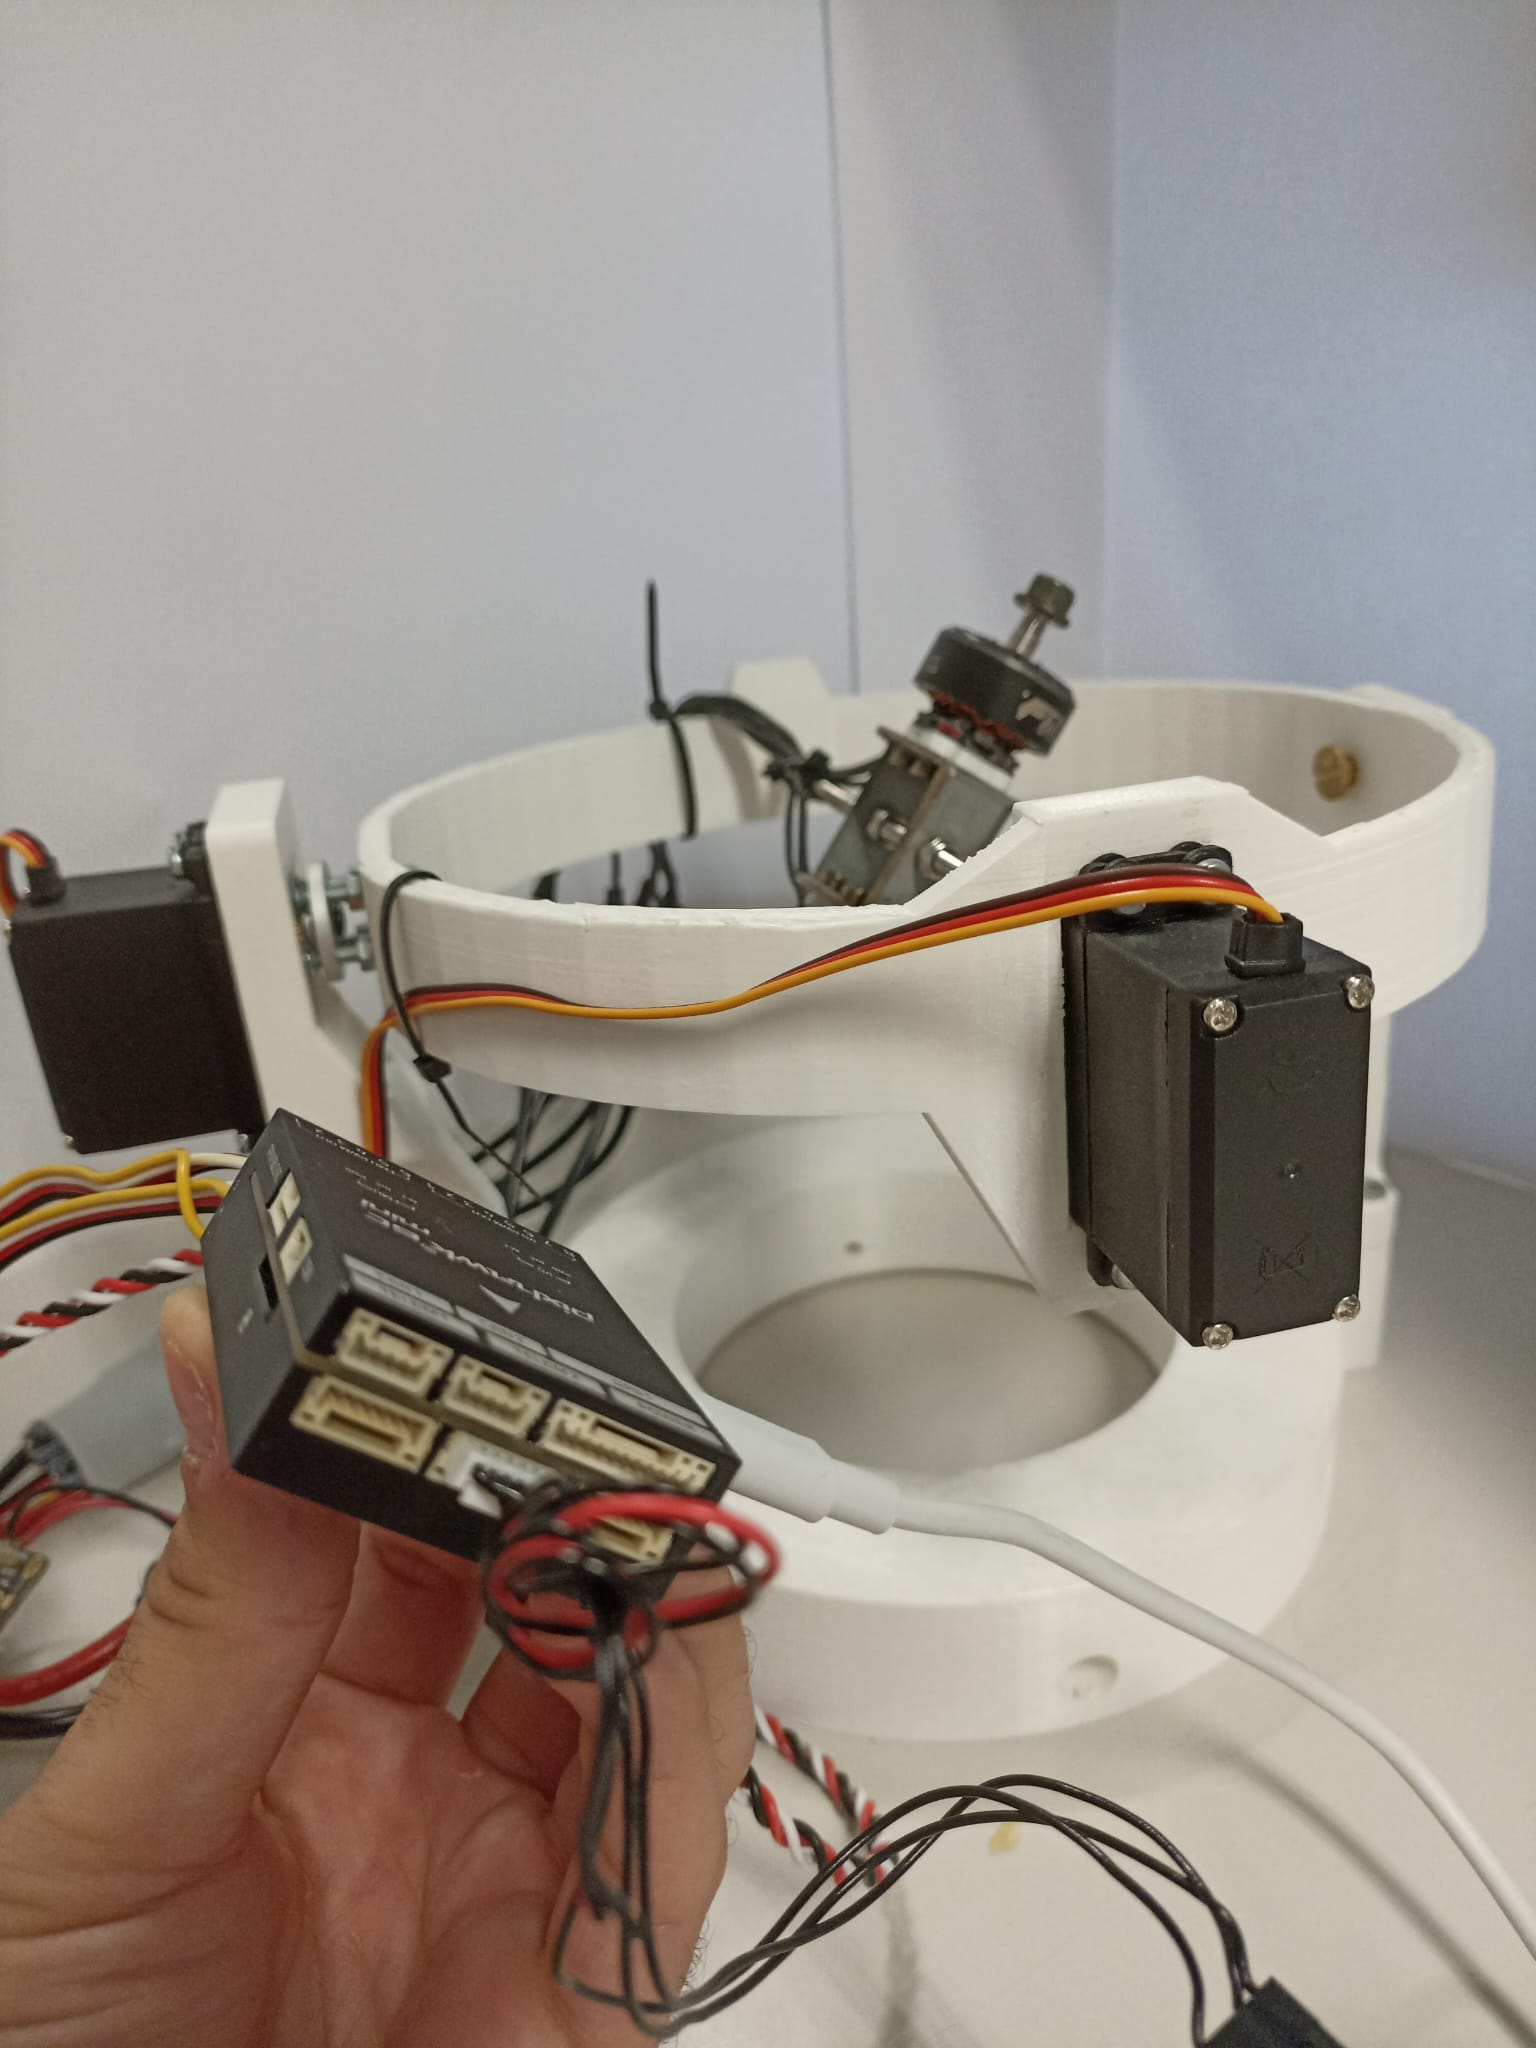
\includegraphics[width=0.23\textwidth]{imgs/demo_tvc/inner_beam_right.jpg}
    }
    \caption{Outer Ring and Inner Beam corresponding to the PX4 attitude}%
\end{figure}

The servos are following the attitude of the vehicle, and are able to control the TVC mechanism.

\clearpage
\section{Conclusion}

In this report we have demonstrated that an offboard computer running ROS 2 can reliably interface with a PX4 flight controller over uXRCE‑DDS to read real‑time attitude estimates and command both servos and motors. 
By implementing a simple state machine and heartbeat protocol, the offboard node successfully:

\begin{itemize}
    \item Switched the flight controller into Offboard mode and armed/disarmed it. 
    \item Subscribed to the VehicleAttitude uORB topic and converted quaternion measurements into servo setpoints. 
    \item Published ActuatorServos and ActuatorMotors messages to drive a thrust‑vectoring mechanism. 
\end{itemize}

Experimental results—including live video, PWM logs, and attitude plots—confirm that the servos tracked the vehicle’s roll/pitch angles within the expected range and the two counter‑rotating motors followed out‑of‑phase commands as intended. This validates the feasibility of using PX4 + ROS 2 offboard control for custom actuation schemes such as TVC.

Future work will extend this framework to closed‑loop control by feeding sensor feedback directly into guidance algorithms and creating a state machine that's syncronized with PX4. Moreover, further safety features (pre‑arm checks, failsafe transitions) and higher‑frequency control loops may be added to meet more demanding control objectives.  

Overall, this demonstration fulfills the primary objective of proving end‑to‑end offboard control of PX4 hardware. 

\clearpage
\section{Appendix}

\label{code::offboard_control.cpp}
\lstinputlisting[language=C++, caption=OffboardControl.cpp]{code/offboard_control.cpp}



%%%%%%%%%%%%%
%    END    %
%%%%%%%%%%%%%

\end{document}
